\documentclass{article}
\usepackage[utf8]{inputenc}
\usepackage{authblk}
\usepackage{setspace}
\usepackage[margin=1.25in]{geometry}
\usepackage{graphicx}
\graphicspath{ {./figures/} }
\usepackage{subcaption}
\usepackage{amsmath}
\usepackage{lineno}
\graphicspath{ {./figures/} }
\usepackage{indentfirst}
\usepackage{graphicx}


%%%%%% Bibliography %%%%%%
% Replace "sample" in the \addbibresource line below with the name of your .bib file.
\usepackage[style=nejm, 
citestyle=numeric-comp,
sorting=none]{biblatex}
\addbibresource{sample.bib}
\title{CS180 Finals Study Guide}

\author{Harris Doan}

\date{June 6, 2023}

%%%%%% Spacing %%%%%%
% Use paragraph spacing of 1.5 or 2 (for double spacing, use command \doublespacing)
\onehalfspacing

\begin{document}

\maketitle

%%%%%% Main Text %%%%%%

\section{Chapter 5: Divide and Conquer}

%%%%% A First Recurrence: The Mergesort Algorithm %%%%%%
\subsection{A First Recurrence: The Mergesort Algorithm}

To motivate the general approach to analyzing divide-and-conquer algorithms, we begin with the \emph{Mergesort} Algorithm. 
To analyze the running time of Mergesort, we will abstract its behavior into the following template, which describes many common divide-and-conquer algorithms.

\medskip 

\emph{(+) Divide the input into two pieces of equal size; solve the two subproblems on these pieces separately by recursion; and then combine the two results into an overall solution, spending only linear time for the initial division and final recombining.}

In Mergesort, as in any algorithm that fits this style, we also need a base case for the recursion, typically having it "bottom out" on inputs of some constant size. In the case of Mergesort, we will assume that once the input has been reduced to size 2, we stop the recursion and sort the two elements by simply comparing them to each other.

\medskip
Consider any algorithm that fits the pattern in (+), and let T(n) denote its worst-case running time on input instances of size n. Supposing that n is even, the algorithm spends O(n) time to divide the input into two pieces of size n/2 each; it then spends time T(n/2) to solve each one (since T(n/2) is the worst-case running time for an input of size n/2); and finally it spends O(n) time to combine the solutions from the two recursive calls. Thus the running time T(n) satisfies the following recurrent relation:

\medskip

For some constant c, 

\medskip

\begin{center}
    T(n) $\le$ 2T(n/2) + cn
\end{center}

\medskip

when n $>$ 2, and

\medskip

\begin{center}
    T(2) $\le$ c
\end{center}

\medskip

The structure is typical of what recurrences will look like: there's an inequality or equation that bounds T(n) in terms of an expression involving T(k) for smaller values k; and there is a base case that generally says that T(n) is equal to a constant when n is a constant. Note that one can also write more informally as T(n) $\le$ 2T(n/2) + O(n), suppressing the constant c. However, it is generally useful to make c explicit when analyzing the recurrence.
\medskip
To keep the exposition simpler, we will generally assume that parameters line n are even when needed. This is somewhat imprecise usage; without this assumption, the two recursive calls would be on problems of size $\lceil n/2 \rceil$ and $\lfloor n/2 \rfloor$, and the recurrence relation would say that
\medskip
\begin{center}
    T(n) $\le$ T($\lceil n/2 \rceil$ + T($\lfloor n/2 \rfloor$) + cn
\end{center}

\subsection{Unrolling the Mergesort Recurrence}

Let's start with the first approach to solving the recurrence. The basic argument is depicted in figure 5.1

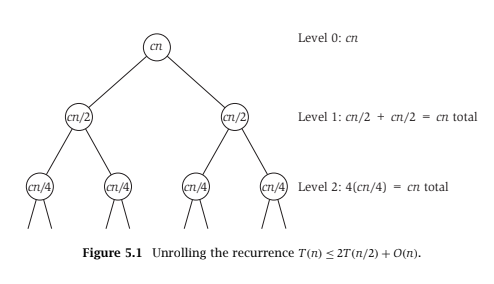
\includegraphics[]{figures/fig1.png}

\medskip

\emph{Analyzing the first few levels}: At the first level of recursion, we have a single problem of size n, which takes time at most cn plus the time spent in all subsequent recursive calls. At the next level, we have two problems each of size n/2. Each of these takes time at most cn/2, for a total of at most cn, again plus the time in subsequent recursive calls. At the third level, we have four problems each of size n/4, each taking time at most cn/4, for a total of at most cn.

\medskip


\emph{Identifying a pattern}: What's going on in general? At level j of the recursion, the number of subproblems has doubled j times, so there are now a total of $2^j$. Each has correspondingly shrunk in size by a factor of two j times, and so each has size n/$2^j$, and hence each takes time at most cn/$2^j$. Thus level j contributes a total of at most $2^j$(cn/$2^j$) = cn to the total running time.

\medskip

\emph{Summing over all levels of recursion}: We've found that the recurrence in 5.1 has the property that the same upper bound of cn applies to total amount of work performed at each level. The number of times the input must be halved in order to reduce its size from n to 2 is log$_2$n. So summing the cn work over logn levels or recursion, we get a total running time of O(nlogn).

\medskip

\begin{center}
    \fbox{Any function T(.) satisfying 5.1 is bounded by O(nlogn), when n $>$ 1}
\end{center}

%%%%%% Counting Inversions %%%%%%
\subsection{Counting Inversions}
\subsubsection{The Problem}
A core issue in applications like this is the problem of comparing two rankings. You rank a set of n movies, and then a collaborative filtering system consults its database to look for other people who had "similar" rankings. But how can we measure, numerically, how similar two people's rankings are?

\medskip

Let's consider comparing your ranking and a stranger's ranking of the same set of n movies. A natural method would be to label the movies from 1 to n according to your ranking, then order these labels according to the stranger's ranking, and see how many pairs are "out of order." These "out of orders" are called inversions. Given a sequence of n numbers a$_1$, ... , a$_n$; we will assume that all the numbers are distinct. We want to define a measure that tells us how far this list is from being in ascending order; the value of the measure should be 0 if a$_1$ $<$ a$_2$ $<$ ... a$_n$, and should increase as the numbers become more scrambled. That is if your ranking and the other rankings differ a lot, then the amount of inversions would increase.

\begin{center}
    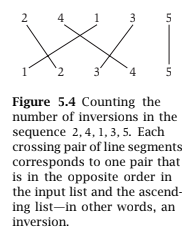
\includegraphics[]{figures/fig2.png}
\end{center}

Looking at Figure 5.4, we can see that we can draw lines from the original sequence to the ascending sequence. Each crossing pair of line segments corresponds to one pair that is in the opposite order in the two lists, which is an inversion.

\subsubsection{Designing the Algorithm}
The simplest way is to compare each element in each ranking, but this would lead to a complexity of O(n$^2$). 

\medskip

We now want to do this in a more efficient manner of O(nlogn) complexity. The basic idea follows the strategy of Mergesort. We set m = $\rceil n/2 \lceil$ and divide the list into two pieces:

\medskip

\begin{center}
    a$_1$, ... , a$_m$ and a$_m+1$ , ... , a$_n$
\end{center}

We first count the number of inversions (a$_i$, a$_j$), where the two numbers belong to different halves; the trick is that we must do this part in O(n) time. The first and second half inversions have a particularly nice form: they are precisely the pair (a$_i$, a$_j$), where a$_i$ is in the first half, a$_j$ is in the second half, and a$_i$ $>$ a$_j$.

\medskip

To help with counting the number of inversions between the two halves, we will make the algorithm recursively sort the numbers in the two halves as well. Having the recursive step do a bit more work (sorting as well as counting inversions) will make the final "combining" portion much easier. Supposed we use function Merge-And-Count and we have recursively sorted the first and second halves of the list and counted the inversions in each. We have a sorted list A and a sorted list B. We want to form a single list C from their union, while also counting the number of pairs (a,b) with a $\in$ A, b $\in$ B, and a $>$ b.

\medskip

It turns out that we will be able to do this in very much the same style that we used for merging. Our Merge-And-Count routine will walk through the sorted list A and list B, removing elements from the front and appending them to the sorted list C. In a given step, we have a \emph{Current} pointer into each list, showing our current position. Suppose that these pointers are currently at element a$_i$ and b$_j$. In one step, we compare the elements, remove the smaller one from its list, and append it to the end of list C.

\medskip

This takes care of merging. \emph{How do we also count the number of inversions?} Because A and B are sorted, it is actually very easy to keep track of the number of inversions we encounter. Each time the element a$_i$ is smaller than everything left in list B, and it comes before all of them. On the other hand, if b$_j$ is append to list C, then it is smaller than all the remaining items in A, and it comes after all of them, so we increase our count of the number of inversions byu the number of elements remaining in A. This is the crucial idea: in constant time, we have accounted for potentially a large number of inversions.\\

\medskip

--------------------------------------------------------------------------------------------------------------------------
\medskip

\textbf{Merge-and-Count(A,B)}\\
Maintain a \emph{Current} pointer into each list, initialized to
point to the front elements\\
Maintain a variable \emph{Count} for the number of inversions,
initialized to 0\\
\texttt{While} both lists are nonempty:\\
\quad Let $a_i$ and $b_j$ be the elements pointed to by the \emph{Current} pointer\\
\quad Append the smaller of these two to the output list\\
\quad If $b_j$ is the smaller element then\\
\quad\quad Increment \emph{Count} by the number of elements remaining in A\\
\quad\texttt{Endif}\\
\quad Advance the \emph{Current} pointer in the list from which the
smaller element was selected.\\
\texttt{EndWhile}\\
Once one list is empty, append the remainder of the other list
to the output\\
Return \texttt{Count} and the merged list

\medskip

--------------------------------------------------------------------------------------------------------------------------
\medskip
\\ 

The running time of Merge-And-Count can be bounded by the analogue of the argument we used for the original merging algorithm at the heart of Mergesort: each iteration of the \texttt{While} loop takes constant time, and in each iteration we add some element to the output that will never be seen again. Thus the number of iterations can be at most the sum of the initial lengths of A and B, and so the total running time is O(n).

\medskip

We use this Merge-And-Count routine in a recursive procedure that simultaneously sorts and counts the number of inversions in a list L.\\

\medskip

--------------------------------------------------------------------------------------------------------------------------
\medskip

\textbf{Sort-And-Count(L)}\\
\texttt{If} the list has one element then\\
there are no inversions\\
\texttt{Else}\\
Divide the list into two halves:\\
A contains the first $\rceil n/2 \lceil$ elements\\
B contains the remaining $\rfloor n/2 \lfloor$ elements\\
(r$_A$, A) = Sort-And-Count(A)\\
(r$_B$, B) = Sort-And-Count(B)\\
(r, L) = Merge-And-Count(A,B)\\
\texttt{Endif}\\
Return r = r$_A$ + r$_B$ + r, and the sorted list L

\medskip

--------------------------------------------------------------------------------------------------------------------------
\medskip
\\

Since our Merge-And-Count procedure takes O(n) time, the running time T(n) of the full Sort-And-Count procedure satisfies the recurrence of 5.1:\\

\medskip


\fbox{\begin{minipage}{12 cm}
The Sort-And-Count algorithm correctly sorts the input list and counts the number of inversions; it runs in O(nlogn) time for a list with n elements.
\end{minipage}}


%%%%%% Finding the Closest Pair of Points %%%%%%
\subsection{Finding the Closest Pair of Points}
\subsubsection{The Problem}
The problem we consider is very simple: Given n points in the plane, find the pair that is closest together. It is immediately clear that there is an O(n$^2$) solution. This solution is compute the distance between each pair of points and take the minimum. It took quite a long time before they resolved this question, and the O(nlogn) algorithm provided is essentially the only one that's been discovered.

\subsubsection{Designing the Algorithm}
Let us denote the set of points by P = {p$_1$, ... , p$_n$}, where p$_i$ has coordinates (x$_i$, y$_i$); and for two points p$_i$, p$_j$ $\in$ P, we use d(p$_i$, p$_j$) to denote the standard Euclidean distance between them. Our goal is to find a pair p$_i$ and p$_j$ that minimizes the distance between those two points. We will also assume that no two points in P have the same x-coordinate or the same y-coordinate.\\

To better visualize this problem, we can imagine the distance of points on a line. How would we find the closet pair of points on a line? We'd first sort them, in O(nlogn) time, and then we'd walk through the sorted list, computing the distance from each point to the one that comes after it. It is easy to see that one of these distances must be the minimum one.\\

Our plan will be to apply divide and conquer used in Mergesort: we find the closest pair among the points in the "left half" of P and the closest pair among the points in the "right half" of P; and then we use this information to get the overall solution in linear time. If we develop an algorithm with this structure, then the solution of our basic recurrence will be O(nlogn).\\

The combing phase of the algorithm is tricky. The distances that have not been considered by either our recursive calls are precisely those that occur between a point in the left half and a point in the right half; there are $\Omega$(n$^2$) such distances, yet we need to find the smallest one in O(n) time. 

\subsubsection{Setting up the Recursion}
Every recursive call, on a set $P^\prime$ $\subseteq$ P, begins with two lists: a list of $P^\prime_x$ in which all the points in $P^\prime$ have been sorted by increasing x-coordinate, and a list $P^\prime_y$ which follows the same pattern. Obviously, we begin with a P$_x$ and P$_y$ list in which we will then sort by increasing x or y coordinates.\\
The first level of recursion: We define Q to be the set of points in the first $\rceil n/2 \lceil$ positions of the left half (P$_x$) and R be the set of points in the first $\rfloor n/2 \lfloor$ positions of the right half (P$_y$). We have effectively created a total of four lists: Q$_x$ = consisting of points in Q sorted by increasing x-coordinates, Q$_y$ = consisting of points in Q sorted by increasing y-coordinates, and analogous lists of R$_x$ and R$_y$. For each entry of each of these lists, as before, we record the position of the point in both lists it belongs to.\\

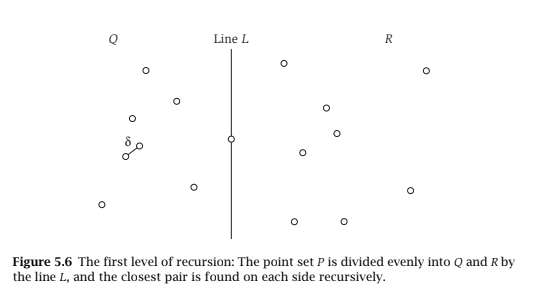
\includegraphics[]{figures/fig3.png}\\

We now recursively determine the closest pair of points in Q (using lists Q$_x$ and Q$_y$). Suppose the correctly returned pair in Q is: (q$^*_0$, q$^*_1$) and the correctly returned pair in R is: (r$^*_0$, r$^*_1$). Now we need to combine the solutions!

\subsubsection{Combining the Solutions}
Let $\delta$ be the minimum of d(q$^*_0$, q$^*_1$) and d(r$^*_0$, r$^*_1$). The real question is: Are there points q $\in$ Q and r $\in$ R for which d(q,r) $<$ $\delta$? If not, then we have already found the closest pair in one of our recursive calls. But if there are, then the closest such q and r form the closest pair in P. This takes into account if the shortest distance is in one half or if they belong in one and the other.\\

\begin{center}
    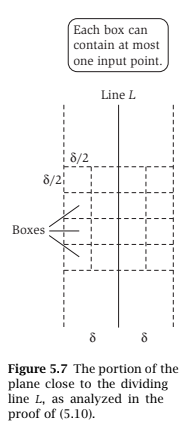
\includegraphics[]{figures/fig4.png}
\end{center}


--------------------------------------------------------------------------------------------------------------------------
\medskip

\textbf{Summary of Algorithm}\\ 
\\
\texttt{Closest-Pair(P)}\\
Construct P$_x$ and P$_y$ (O(nlogn) time)\\
(P$^*_0$, P$^*_1$) = Closest-Pair-Rec(P$_x$, P$_y$)\\
\\
\texttt{Closest-Pair-Rec(P$_x$, P$_y$)}\\
\texttt{If} $|P|$ $\le$ 3 then\\
find closest pair by measuring all pairwise distances\\
\texttt{Endif}\\
\\
\texttt{Construct Q$_x$, Q$_y$, R$_x$, R$_y$} (O(n) time)\\
(q$^*_0$, q$^*_1$) = Closest-Pair-Rec(Q$_x$, Q$_y$)\\
(r$^*_0$, r$^*_1$) = Closest-Pair-Rec(R$_x$, R$_y$)\\
\\
$\delta$ = min(d(q$^*_0$, q$^*_1$), d(r$^*_0$, r$^*_1$))\\
x$^*$ = maximum x-coordinate of a point in set Q\\
L = {(x,y) : x = x$^*$}\\
S = points in P within distance $\delta$ of L.\\
\\
Construct S$_y$ (O(n) time)\\
\texttt{For} each point s $\in$ S$_y$, compute distance from s to each of the next 15 points in S$_y$\\
\texttt{Let} s, $s^\prime$ be pair achieving minimum of these distances (O(n) time)\\
\\
\texttt{If} d(s,$s^\prime$) $<$ $\delta$ then\\
\texttt{Return} (s,$s^\prime$)\\
\texttt{Else if} d(q$^*_0$, q$^*_1$) $<$ d(r$^*_0$, r$^*_1$)\\
\texttt{Return} (q$^*_0$, q$^*_1$)\\
\texttt{Else}\\
\texttt{Return} (r$^*_0$, r$^*_1$)\\
\texttt{Endif}

\medskip

--------------------------------------------------------------------------------------------------------------------------
\medskip

We proved that the algorithm produces the correct answer, using the facts we've established in the process of designing it.\\

\begin{center}
    \fbox{The algorithm correctly outputs a closest pair of points in P}
\end{center}

Proof: As we've noted, all the components of the proof have already been worked out, so here we just summarize how they fit together.\\
We prove the correctness by induction on the size of P, the case of $|P|$ $\le$ 3 being clear. For a given P, the closest pair in the recursive call is computed correctly by induction. The remainder of the algorithm correctly determines whether any pair of points in S is at distance less than $\delta$, and if so returns the closest such pair. Now the closest pair in P either has both elements in one of Q or R, or it has one element in each. In the former case, the closest pair is correctly found by the recursive call; in the latter case, this pair is at distance less than $\delta$ and it is correctly found by the remainder of the algorithm.\\

\begin{center}
    \fbox{The running time of the algorithm is O(nlogn)}
\end{center}


\section{Chapter 6: Dynamic Programming}
 We began our study of algorithmic techniques with greedy algorithms, which in some sense form the most natural approach to algorithm design. Faced with a new computational problem, we’ve seen that it’s not hard to propose multiple possible greedy algorithms; the challenge is then to determine whether any of these algorithms provides a correct solution to the problem in all cases.\\
 
We now turn to a more powerful and subtle design technique, dynamic programming. It will be easier to say exactly what characterizes dynamic programming after we have seen it in action, but the basic idea is drawn from the intuition behind divide and conquer and is essentially the opposite of the greedy strategy: one implicitly explores the space of all possible solutions, by carefully decomposing things into a series of sub-problems, and then building up correct solutions to larger and larger sub-problems.

\subsection{Weighted Interval Scheduling: A Recursive Procedure}
We have seen that a particular greedy algorithm produces an optimal solution to the Interval Scheduling Problem, where the goal is to accept as large a set of non-overlapping intervals as possible. The Weighted Interval Scheduling Problem is a strictly more general version, in which each interval has a certain value (or weight), and we want to accept a set of maximum value.\\

\subsubsection{Designing A Recursive Algorithm}
Since the original Interval Scheduling Problem is simply the special case in which all weights are equal to 1, we know already that the most greedy algorithms will not solve this problem optimally. We will begin our introduction to dynamic programming with a recursive type of algorithm for this problem.\\

\begin{center}
    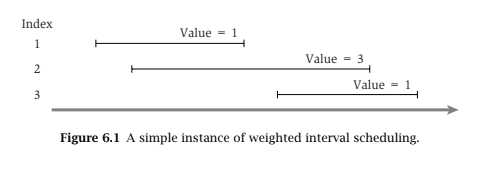
\includegraphics[]{figures/fig5.png}
\end{center}

Using the notation from the original problem, we have n requests labeled 1, ... , n. With each request i specifying a start time s$_i$ and a finish time f$_i$. Each interval i now also has a weight v$_i$. Two intervals are compatible if they do not overlap. The goal of our current problem is to select a subset S $\subseteq$ {1,..,n} of mutually compatible intervals, so as to maximize the sum of the values of the selected intervals $\sum_{ i \in S  }^{}$v$_i$.\\

Let's supposed that the requests are sorted in order of non-decreasing finish time: f$_1$ $\le$ f$_2$ $\le$ ... f$_n$. We'll say a request i comes before a request j if i $<$ j. To help in order, we define p(j), for an interval j, to be the largest index i $<$ j such taht intervals i and j are disjoint. In other words, i is the leftmost interval that ends before j begins. We define p(j) = 0 if no request i $<$ j is disjoint from j.\\

\begin{center}
    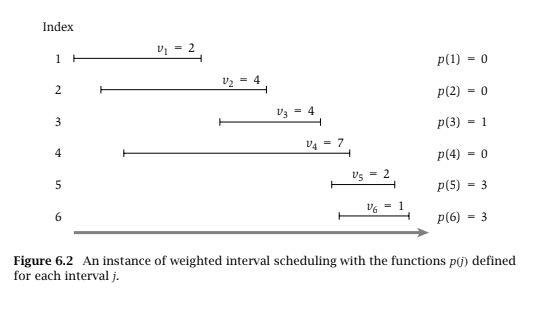
\includegraphics[]{figures/fig6.png}
\end{center}

Now, given an instance of the Weighted Interval Scheduling Problem, let's consider an optimal solution O (ignore for now, since we have no idea what it is). Something obvious we can say: either interval n (the lat one) belongs to O or it doesn't. Supposed we explore both sides of this dichotomy a little further. If n $\in$ O, then clearly no interval indexed strictly between p(n) and n can belong to O, because by the definition of p(n), we know that intervals p(n)+1, p(n)+2, ... , n-1 all overlap interval n. Moreover, if n $\in$ O, then O must include an optimal solution to the problem consisting of requests {1,...,p(n)}. If it didn't, we could replace O's choice of requests from {1,...,p(n)} with a better one, with no danger of overlapping requests n.\\

On the other hand, if n $\notin$ O, then O is simply equal to the optimal solution to the problem, consisting of requests {1,..., n-1}. This is a completely analogous reasoning; we're assuming that O does not include request n; so if it does not choose the optimal set of requests from {1,..., n-1}, we could replace it with a better one.\\

This suggests that the optimal solution on intervals {1,2,...n} involves looking at optimal solutions for smaller problems: {1,...,j} and let opt(j) denote that solution. (We define opt(0) = 0). The optimal solution we're seeking is precisely O$_n$m with the value opt(n). For the case of the optimal solution O$_j$, our reasoning above says that either j $\in$ O$_j$ or j $\notin$ O$_j$.\\

\begin{center}
    \fbox{j $\in$ O$_j$ = opt(j) = v$_j$ + opt(p(j))}
\end{center}

\begin{center}
    \fbox{j $\notin$ O$_j$ = opt(j-1)}
\end{center}

We can further conclude since there are only two possibilities:

\begin{center}
    \fbox{opt(j) = max(v$_j$ + opt(p(j)), opt(j-1))}
\end{center}

And how we decide whether n belongs to the optimal solution O$_j$? It belongs to the optimal solution if and only if the first of the options above is at least as good as the second:

\begin{center}
    \emph{Request j belongs to an optimal solution on set {1,2..,j} if and only if}\\
    \fbox{v$_j$ + opt(p(j)) $\ge$ opt(j-1)}
\end{center}

These facts form the first crucial component on which a dynamic programming solution is based: a recurrence equation that expressed the optimal solution in terms of then optimal solutions to smaller sub-problems.\\

\medskip

--------------------------------------------------------------------------------------------------------------------------
\medskip

\textbf{Compute-Opt(j)}
\texttt{If} j = 0 then\\
\texttt{Return} 0\\
\texttt{Else}\\
\texttt{Return} max(v$_j$ + Compute-Opt(p(j)), Compute-Opt(j-1))\\
\texttt{Endif}\\

\medskip

--------------------------------------------------------------------------------------------------------------------------
\medskip

\begin{center}
    \fbox{Compute-Opt(j) correctly computes opt(j) for each j = 1,2, ..., n}
\end{center}

Unfortunately, if we really implemented the algorithm Compute-Opt as is, it would take exponential time to run in the worst case. The total number of calls made to Compute-Opt on this instance will grow like the Fibonacci numbers, which increases exponentially. Thus we have not achieve polynomial time.\\

\begin{center}
    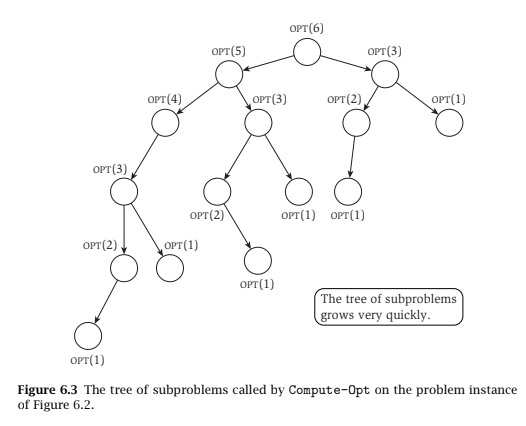
\includegraphics[]{figures/fig7.png}
    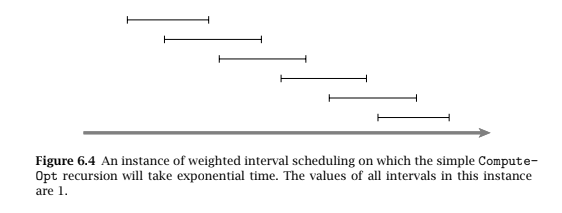
\includegraphics[]{figures/fig8.png}
\end{center}

\subsubsection{Memoizing The Recursion}
Our solution is really only solving n+1 different sub-problems: Compute-Opt(0), Compute-Opt(1),..,Compute-Opt(n). How can we remove the redundancy? We could store the value of Compute-Opt in a globally accessible place the first time we compute it and then simply use it in place of all future recursive calls. This is called memoization.

\medskip

--------------------------------------------------------------------------------------------------------------------------
\medskip

\textbf{M-Compute-Opt(j)}\\
\texttt{If} j = 0 then\\
\texttt{Return} 0\\
\texttt{Else if} M[j] is not empty then\\
\texttt{Return} M[j]\\
\texttt{Else}\\
\texttt{Define} M[j] = max(v$_j$ + M-Compute-Opt(p(j)), M-Compute-Opt(j-1))\\
\texttt{Return} M[j]\\
\texttt{Endif}\\

\medskip

--------------------------------------------------------------------------------------------------------------------------
\medskip

\begin{center}
    \fbox{The running time of M-Compute-Opt(n) is O(n) (assuming the input intervals are sorted by their finish times)}
\end{center}

\subsubsection{Computing a Solution in Addition to Its Value}
So far we have simply computed the value of an optimal solution in addition to its value. We don't want to maintain the set by explicitly defining a set in the S array. This would take O(n) time, but would blow up since we are not explicitly maintaining S. Instead we can recover the optimal solution from values saved in the array M after the optimum value has been computed. 

\medskip

--------------------------------------------------------------------------------------------------------------------------
\medskip

\textbf{Find-Solution(j)}\\
\texttt{If} j = 0 then\\
\texttt{Output} nothing\\
\texttt{Else}\\
\texttt{If} v$_j$ + M[p(j)] $\ge$ M[j-1] then
\texttt{Output} j together with the result of Find-Solution(p(j))\\
\texttt{Else}\\
\texttt{Output} the result of Find-Solution(j-1)\\
\texttt{Endif}\\
\texttt{Endif}\\
 
\medskip

--------------------------------------------------------------------------------------------------------------------------
\medskip

Since Find-Solution calls itself recursively only on strictly smaller values, it makes a total of O(n) recursive calls; and since it spends constant time per call; we have:\\

\fbox{\begin{minipage}{12 cm}
Given the array M of the optimal values of the sub-problems, Find-Solution returns an optimal solution in O(n) time.
\end{minipage}}

\subsubsection{Principles of Dynamic Programming: Memoization or Iteration Over Sub-problems}
We now use the algorithm for the Weighted Interval Scheduling Problem developed in the previous section to summarize the basic principles of dynamic programming, and also to offer a different perspective that will be fundamental to the rest of the chapter: iterating over sub-problems, rather than computing solutions recursively.\\

\subsubsection{Designing the Algorithm}
The key to the efficiency of the algorithm is really the array M. The point is to realize that we can directly compute the entries in M by an iterative algorithm, rather than using memoized recursion. We just start with M[0] = 0 and keep incrementing j; each time we need to determine a value M[j], the algorithm looks like:\\

\medskip

--------------------------------------------------------------------------------------------------------------------------
\medskip

\textbf{Iterative-Compute-Opt}\\
M[0] = 0\\
\texttt{For} j = 1,2,...,n\\
M[j] = max(v$_j$ + M[p(j)], M[j-1])\\
\texttt{Endfor}\\

 
\medskip

--------------------------------------------------------------------------------------------------------------------------
\medskip

\subsubsection{Analyzing the Algorithm}
By exact analogy, we can prove by induction on j that this algorithm writes opt(j) in array entry M[j]. Also, we can pass the filled-in array M to Find-Solution to get an optimal solution in addition to the value. Finally, the running time of Iterative-Compute-Opt is clearly O(n), since it explicitly runs for n iterations and spends constant time in each.\\

\subsection{A Basic Outline of Dynamic Programming}
The two approaches clearly have a great deal of conceptual overlap, since they both grow from the insight contained in the recurrence. we will develop dynamic programming algorithms using the second type of approach—iterative building up of sub-problems because the algorithms are often simpler to express this way. But in each case that we consider, there is an equivalent way to formulate the algorithm as a memoized recursion.\\

To set about developing an algorithm based on dynamic programming, one needs a collection of sub-problems derived from the original problem that satisfies a few basic properties.

\begin{figure}[htbp]
    \centering
    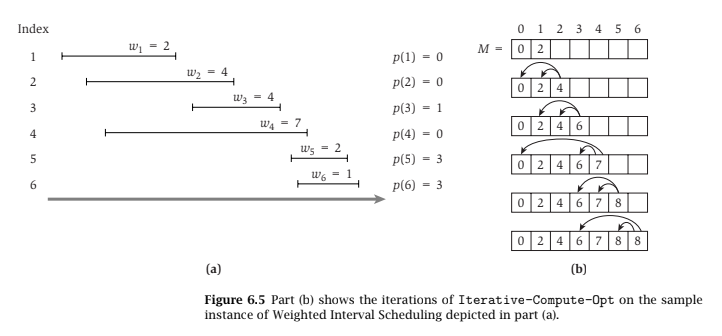
\includegraphics[width=\textwidth]{figures/fig9.png}
\end{figure}

\begin{enumerate}
    \item There are only a polynomial number of sub-problems
    \item The solution to the original problem can be easily computed from the solutions to the sum-problems. (i.e, the original problem may actually be one of the sub-problems)
    \item There is a natural ordering on sub-problems from "smallest" to "largest," together with an easy-to-compute recurrence and that allows one to determine the solution to a sub-problem from the solutions to some number of smaller sub-problems.
\end{enumerate}

We will see that it is sometimes easier to start the process of designing such an algorithm by formulating a set of sub-problems that looks natural, and then figuring out a recurrence that links them together; but often it can be useful to first define a recurrence by reasoning about the structure of an optimal solution, and then determine which sub-problems will be necessary to unwind the recurrence.\\

\subsection{Segmented Least Squares: Multi-way Choices}
In the previous section, our choices in the recurrence was binary. It was either in or out. However, there are problems in which we have to consider a recurrence that involves a polynomial number of possibilities. We can call this a "multi-way choice" and at each step we have a polynomial number of possibilities to consider.\\

\subsubsection{The Problem}
Often when looking at scientifc or statistical data, plotted on a two-dimensional set of axes, one tries to pass a "line of best fit" through the data. This is the foundational problem in statistics and numerical analysis, formulated as follows.\\

Supposed our data consists of a set P of n points in the plane, denoted (x$_1$, y$_1$), (x$_2$, y$_2$), ... , (x$_n$, y$_n$); and supposed x$_1$ $<$ x$_2$ $<$ ... x$_n$. Given a line L defined by the equation y = ax+b, we say that the error of L with respect to P is the sum of its squared "distances" to the points in P:

\begin{center}
   Error(L,P) = $\sum_{i = 1}^{n}$ (y$_i$ - ax$_i$ - b)$^2$
\end{center}

\begin{center}
    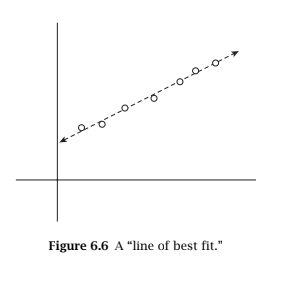
\includegraphics[]{figures/fig10.png}
\end{center}

\begin{center}
    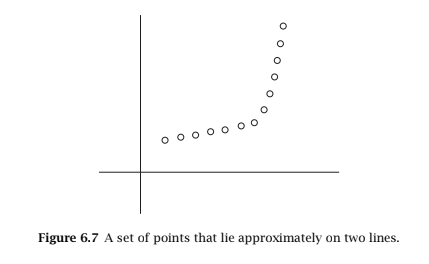
\includegraphics[]{figures/fig11.png}
\end{center}

A natural goal is then to find the line with minimum error. This can actually be derived with Calculus. The line of minimum error is y = ax + b, where:\\

\begin{center}
    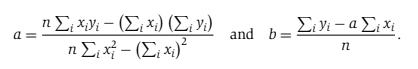
\includegraphics[]{figures/fig12.png}
\end{center}

One extreme of attacking this problem is instead of seeking a single line of best fit, instead to pass an arbitrary set of lines through the points and seek to minimize the error. But this fails as a good problem formulation, because it has a trivial solution. At the other extreme, we could try "hard-coding" the number two into the problem; we could seek the best fit using at most two lines, but this misses a crucial feature of our intuition. We didn't start out with a preconceived idea that the points lay approximately on two lines; we concluded that from looking at the picture. So we have no clue of knowing how the points are laid out.

\begin{center}
    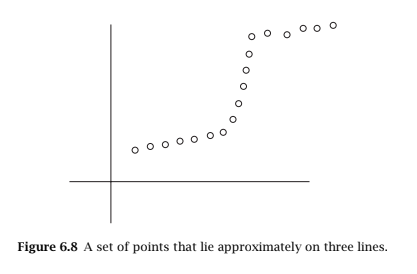
\includegraphics[]{figures/fig13.png}
\end{center}

Thus, the problem that formulation that fits our criteria is the \emph{Segmented Least Squares Problem}. This captures these issues quite cleanly. The problem is a fundamental instance of an issue in data mining and statistics known as \emph{change detection}: Given a sequence of data points, we want to identify a few points in the sequence a which a discrete change occurs.\\

\subsubsection{Design the Algorithm}
For segmented least squares, the following observation is very useful: The last point P$_n$ belongs to a single segment in the optimal partition, and that segments begins at some earlier point p$_i$. This is the type of observation that can suggest the right set of sub-problems; if we knew the identity of the last segment (p$_1$,...,p$_n$), then we could remove those points from consideration and recursively solve the problem on the remaining points: (p$_1$,...,p$_i-1$).\\

\begin{center}
    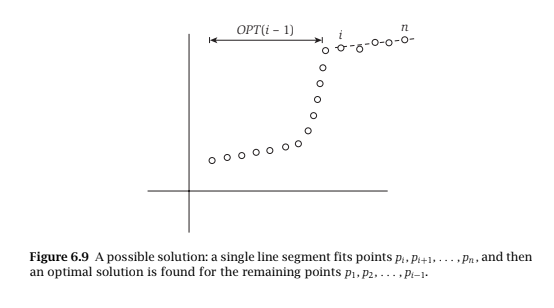
\includegraphics[]{figures/fig14.png}
\end{center}

Suppose we let opt(i) denote the optimum solution for the points (p$_1$,...,p$_i$), and we let e$_i,j$ denote the minimum error of any line with respect to (p$_i$, p$_i+1$ ,...,p$_j$). We will write opt(0) = 0 as a base case. Then our observation above says the following:\\

\fbox{\begin{minipage}{12 cm}
If the last segment of the optimal partition is p$_i$, ... , p$_n$, then the value of the optimal solution is opt(n) = e$_i,n$ + C + opt(i-1).
\end{minipage}}\\

Using the same observation for the sub-problem consisting of points p$_1$, ... , p$_j$, we see that to get to opt(j) we should find the best way to produce the final segment p$_i$, ... , p$_j$. Paying the error plus the additive C for this segment, together with the optimal solution opt(i-1) for the remaining points. In other words, we have justified the following recurrence.\\

\fbox{\begin{minipage}{12 cm}
(6.7)\\
For the sub-problem on the points p$_1$, ... , p$_j$,\\

\begin{center}
    opt(j) = min(e$_i,j$ + C + opt(i-1)), where min: 1 $\le$ i $\le$ j\\
\end{center}
and the segment p$_i$, ... , p$_j$ is used in an optimum solution for the sub-problem if and only if the minimum is obtained using index i.
\end{minipage}}

\medskip
--------------------------------------------------------------------------------------------------------------------------
\medskip

\textbf{Segmented-Least-Squares(n)}\\
Array M[0...n]\\
\texttt{Set} M[0] = 0\\
\texttt{For} all pairs i $\le$ j\\
Compute the least squares error e$_i,j$ for the segment p$_i$, ... , p$_j$\\
\texttt{Endfor}\\
\texttt{For} j = 1,2,...,n \\
Use the recurrence (6.7) to compute M[j]\\
\texttt{Endfor}\\
\texttt{Return} M[n]


 
\medskip
--------------------------------------------------------------------------------------------------------------------------
\medskip

Same as the weighted interval scheduling problem, we can trace back through the array M to compute the optimum partition:\\

\medskip
--------------------------------------------------------------------------------------------------------------------------
\medskip

\textbf{Find-Segments(j))}\\
\texttt{If} j = 0, then\\
Output nothing\\
\texttt{Else}\\
Find an i that minimizes e$_i,j$ + C + M(i-1)\\
Output the segment {p$_i$, ... , p$_j$} and the result of\\
Find-Segments(i-1)\\
\texttt{Endif}

 
\medskip
--------------------------------------------------------------------------------------------------------------------------
\medskip

\subsubsection{Analyzing the Algorithm}
Considering the run time, first we need to compute the values of all the least-squares error e$_i,j$. Note that there are O(n$^2$) pairs (i,j) that are needed for the calculation. Using the formula given at the beginning of the section to compute e$_i,j$ in O(n) time. Thus the total running time to compute the least-squares error is O(n$^3$).\\

This algorithm has n iterations, for values j = 1,2,...,n. For each j, we have to determine the minimum in the recurrence to fill in the array M[j]; which takes O(n) time. This is a total of O(n$^2$). Thus the running time is O(n$^2$) once all the e$_i,j$ values have been determined.

\subsection{Subset Sums and Knapsacks: Adding a Variable}
So far we’ve considered problems in which requests are specified by a given interval of time on a resource, as well as problems in which requests have a duration and a deadline but do not mandate a particular interval during which they need to be done. In this section, we consider a version of the second type of problem, with durations and deadlines, which is difficult to solve directly using the techniques we’ve seen so far. We will use dynamic programming to solve the problem, but with a twist: the “obvious” set of sub-problems will turn out not to be enough, and so we end up creating a richer collection of sub-problems. As we will see, this is done by adding a new variable to the recurrence underlying the dynamic program.\\

\subsubsection{The Problem}
In the scheduling problem we consider here, we have a single machine that can process jobs, and we have a set of requests {1, 2, . . . , n}. We are only able to use this resource for the period between time 0 and time W, for some number W. Each request corresponds to a job that requires time w$_i$ to process. If our goal is to process jobs so as to keep the machine as busy as possible up to the “cut-off” W, which jobs should we choose?\\

\textbf{Subset Sum Problem}
\begin{enumerate}
    \item We are given n items: {1,..., n}
    \item Each has a non-negative weight w$_i$ (for i = 1,...,n)
    \item We are given a bound W
\end{enumerate}

\textbf{Goal}: We want to select a subset S such that \begin{center}
    \fbox{if n $\notin$ O, then opt(n) = opt(n-1)}
\end{center} w$_i$ $\le$ W\\

This problem is a natural special case of a more general problem called the \emph{Knapsack Problem}, where each request i has both a value v$_i$ and a weight w$_i$. The goal being to select a subset of maximum total value, subject to the restriction of W. The knapsack refers to the problem of filling a knapsack with a capacity W as full as possible, using a subset of items {1,..,n}.\\

Since this resembles a greedy type question, can greedy find an optimal solution? The answer is no. We think we could sort by decreasing weight, however a case where W is a multiple of 2 would lead to a non-optimal solution. If we sort by increasing weight, inputs such as {1, W/2, W/2} would fail. The tricky issue here is figuring out a good set of sub-problems.

\subsubsection{Designing the Algorithm}
\textbf{A False Start}: One general strategy, is to consider sub-problems involving only the first i requests. Our strategy was to imagine an optimal solution O and whether or not the last request n is $\in$ or $\notin$ O. With this definition of opt(i):\\

\begin{center}
    \fbox{if n $\notin$ O, then opt(n) = opt(n-1)}
\end{center}

Next, consider that: n $\in$ O. Unlike the weighted interval scheduling problem, we can't just delete each request since for a request n, it has a weight w$_n$. If we accept this request n then we only have W - w$_n$ weight left for the remaining elements in the set S that we can potentially accept.\\

\textbf{A Better Solution}: We need more sub-problems! To find out the value of opt(n) we not only need opt(n-1), we also need to know the best solution we can get using a subset of the first (n-1) items and total allowed weight W - w$_n$. Therefore, we are going to use a lot more sub-problems: one for each initial set {1,...,i} of the items, and each possible value for the remaining available weight w.\\

\begin{center}
    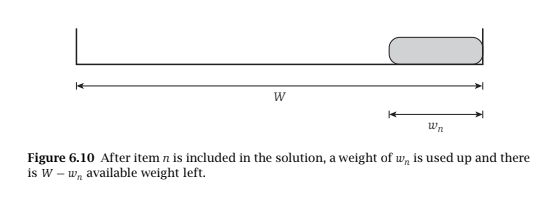
\includegraphics[]{figures/fig15.png}
\end{center}

Assume that W is an integer, and all requests i = 1,...,n and have weights w$_i$. We will have a sub-problem for each i = 0,1,..,n and each integer 0 $\le$ w $\le$ W. We will use opt(i,w) to denote the value of the optimal solution using a subset of items {1,...,i} with the maximum allowed weight w:

\begin{center}
    opt(i,w) = max$_s$ $\sum_{j \in S}^{}$ W$_j$,
\end{center}

The maximum is over subsets S $\subseteq$ {1,...,i} that satisfies $\sum_{j \in S}^{}$ W$_j$ $\le$ w. Using this new set of sub-problems, we will be able to express the value opt(i,w) as a simple expression in terms of values from smaller problems. Moreover, opt(n,W) is the quantity we're looking for in the end. As before, let O denote an optimum solution for the original problem.\\

\begin{enumerate}
    \item We are given n items: {1,..., n}
    \item If $\in$ O, then opt(n, W) = w$_n$ + opt(n - 1, W - w$_n$), since we now seek to use remaining capacity of W - w$_n$ in an optimal way across items 1,2,...,(n-1).
\end{enumerate}

When the n$^th$ item is too big, that is, W $<$ w$_n$, then we must have opt(n, W) = opt( n-1, W). Otherwise, we get the optimum solution allowing all n requests by taking the better of these two options. Using the same line of argument for the sub-problem for items {1,...,i}, and maximum allowed weight w, gives us the following recurrence.\\

\fbox{\begin{minipage}{12 cm}

\begin{center}
(6.8)\\
if w < w$_i$ then opt(i,w) = opt(i-1, w). Otherwise\\
opt(i,w) = max(opt(i-1, w), w$_i$ + opt(i-1, w-w$_i$))
\end{center}

\end{minipage}}

As before, we want to design an algorithm that builds up a table of all opt(i,w) values while computing each of them at most once.

\medskip
--------------------------------------------------------------------------------------------------------------------------
\medskip

\textbf{Subset-Sum{n,W}}\\
Array M[0...n, 0...W]\\
\texttt{Initialize} M[0,w] = 0 for each w = 0,1,...,W\\
\texttt{For} i = 1,2,..,n\\
\texttt{For} w = 0,...,W\\
Use the recurrence (6.8) to compute M[i,w]\\
\texttt{Endfor}\\
\texttt{Endfor}\\
\texttt{Return} M[n,W]

\medskip
--------------------------------------------------------------------------------------------------------------------------
\medskip

\begin{center}
    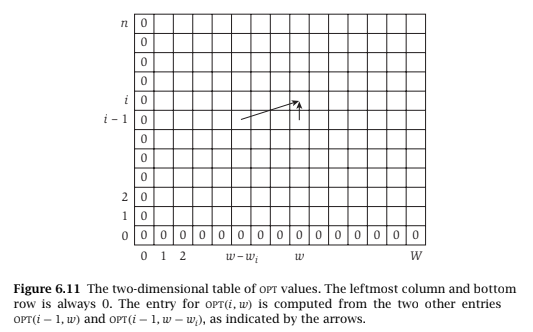
\includegraphics[]{figures/fig16.png}
\end{center}

\subsubsection{Analyzing the Algorithm}
For the algorithm we've just designed, we can use a similar representation, but we need a 2D table, reflecting the 2D array of sub-problems that is being built up. The figure below shows the building up of sub-problems in this case: the value M[i,w] is computed from the two other values M[i-1, w] and M[i-1, w - w$_i$]. Next we will worry about the running time of this algorithm. As before in the case of weighted interval scheduling, we are building up a table of solutions M, and we compute each of the values M[i,w] in O(1) time using the previous values. Thus the running time is proportional to the number of entries in the table.\\

\begin{center}
    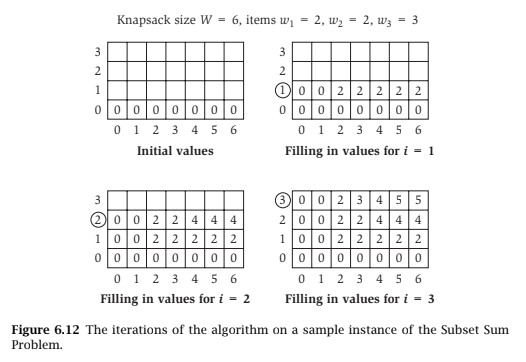
\includegraphics[]{figures/fig17.png}
\end{center}


\fbox{\begin{minipage}{12 cm}

\begin{center}
The Subset-Sum(n,W) Algorithm correctly computes the optimal value of the problem, and runs in O(nW) time.
\end{center}

\end{minipage}}

Note that this method is not as efficient as our dynamic program for the weighted interval scheduling. The running time is not a polynomial function of n; rather it is a polynomial function of n and W, the largest integer involved in defining the problem. We call such algorithms pseudo-polynomial. Pseudo-polynomial algorithms can be reasonably efficient when the numbers {W$_i$} involved in the input are reasonably small; however, they become less practical as numbers grow larger. To recover an optimal set S of items, we can trace back through the array M by a procedure similar to those we developed in the previous statements.

\fbox{\begin{minipage}{12 cm}

\begin{center}
Given a table M of the optimal values of the sub-problems, the optimal set S can be found in O(n) time.
\end{center}

\end{minipage}}

\subsubsection{The Knapsack Problem}
\textbf{Goal}: The goal is to find a subset S of a maximum value $\sum_{i \in S}^{}$ v$_i$, subject to the restriction that the total weight of the set should not exceed W: $\sum_{i \in S}^{}$ w$_i$ $\le$ W.\\

We now consider an optimal solution O, and identify two cases depending on whether or not it belongs to the optimal solution:\\

\begin{enumerate}
    \item if n $\notin$ O, then opt(n,W) = opt(n - 1, W)
    \item if n $\in$ O, then opt(n,W) = v$_n$ + opt(n - 1, W - w$_n$)
\end{enumerate}

\fbox{\begin{minipage}{12 cm}

\begin{center}
if w $<$ w$_i$ then opt(i, w) = opt(i - 1, w). Otherwise\\
opt(i,w) = max(opt(i - 1, w), v$_i$ + opt(i - 1, w - w$_i$)
\end{center}

\end{minipage}}\\

Using this recurrence, we can write down a completely analogous dynamic programming algorithm, and this implies the following:\\

\begin{center}
    \fbox{The Knapsack Problem can be solved in O(nW) time.}
\end{center}

\subsubsection{RNA Secondary Structure: Dynamic Programming over Intervals}
There are a few canonical problems that fit this profile; those of you who have studied parsing algorithms for context-free grammars have probably seen at least one dynamic programming algorithm in this style. Here we focus on the problem of RNA secondary structure prediction, a fundamental issue in computational biology.

\subsubsection{The Problem}
As one learns in introductory biology classes, Watson and Crick posited that double-stranded DNA is “zipped” together by complementary base-pairing. Each strand of DNA can be viewed as a string of bases, where each base is drawn from the set {A, C, G, T}. A-T pair and C-G pair. However, unlike double-stranded DNA, there’s no “second strand” for the RNA to stick to; so it tends to loop back and form base pairs with itself, resulting in interesting shapes. The set of pairs (and resulting shape) formed by the RNA molecule through this process is called the secondary structure, and understanding the secondary structure is essential for understanding the behavior of the molecule.\\

For our purposes, a single-stranded RNA molecule can be viewed as a sequence of n symbols (bases) drawn from the alphabet (A,C,G,U). Let B = b$_1$, b$_2$, ... b$_n$ be a single stranded RNA molecule, where b$_i$ $\in$ {A,C,G,U}. We require A-U, C-G, and each base can pair with at most one other base. The set of base pairs forms a \emph{matching}. It also turns out that secondary structure are "knot-free," which will formalize as a kind of non-crossing behavior.\\

Thus we can say that a secondary structure on B is a set of pairs S = {(i,j)}, where i,j $\in$ {1,2,...n}, that satisfies the following conditions:\\

\begin{enumerate}
    \item (no sharp turns) The ends of each pair in S are separated by at least four intervening bases; that is, if (i,j) $\in$ S, then i $<$ j -4
    \item The elements of any pair in S consist of either {A,U} or {C,G} (in either order)
    \item S is a matching: no base appears in more than one pair
    \item (the non-crossing condition) If (i,j) and (k,l) are two pairs in S, then we cannot have i $<$ k $<$ j $<$ l.
\end{enumerate}

\begin{center}
    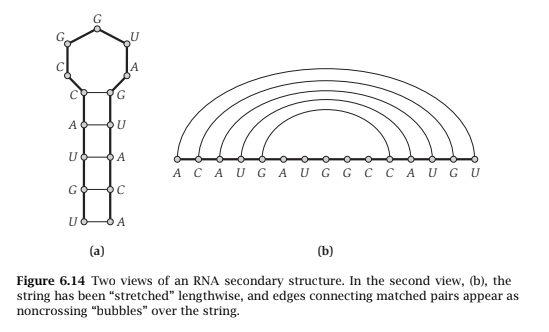
\includegraphics[]{figures/fig18.png}
\end{center}

\subsubsection{Designing and Analyzing the Algorithm}
\textbf{A First Attempt at Dynamic Programming}: We say that opt(j) is the maximum number of base pairs in a secondary structure on b$_1$, b$_2$, ... , b$_j$. By the no-sharp-turns condition above, we know that opt(j) = 0 for j $\le$ 5; and we know that opt(n) is the solution we're looking for. The trouble comes when we try writing down a recurrence that expresses opt(j) in terms of the solutions to smaller sub-problems. We can get partway there: in the optimal secondary structure b$_1$, b$_2$, ... , b$_j$, it's the case that either:\\

\begin{enumerate}
    \item j is not involved in a pair; or
    \item j pairs with t some t $<$ j-4
\end{enumerate}

\begin{center}
    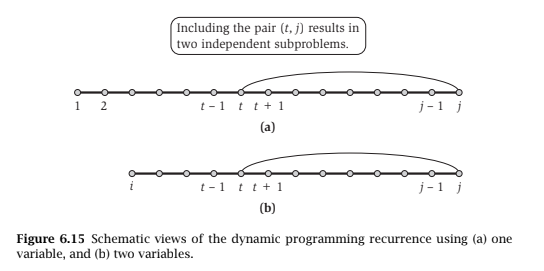
\includegraphics[]{figures/fig19.png}
\end{center}

\textbf{Dynamic Programming over Intervals}: Let opt(i,j) denote the maximum number of base pairs in a secondary structure on b$_i$, b$_i+1$, ... , b$_j$. The no-sharp-turns condition lets us initialize opt(i,j) = 0 whenever i $\ge$ j-4. Now in the optimal secondary structure on b$_i$, b$_i+1$, ... , b$_j$, we have the same alternatives as before:\\

\begin{enumerate}
    \item j is not involved in a pair; or
    \item j pairs with t some t $<$ j-4
\end{enumerate}

\fbox{\begin{minipage}{12 cm}

\begin{center}
(6.13)\\
opt(i,j) = max(opt(i, j-1), max(1+ opt(i, t - 1) + opt(t + 1, j -1))), where the max is taken over t such that b$_t$ and b$_j$ are an allowable base pair (under conditions (i) and (ii) from the definition of a secondary structure).
\end{center}

\end{minipage}}\\

\begin{center}
    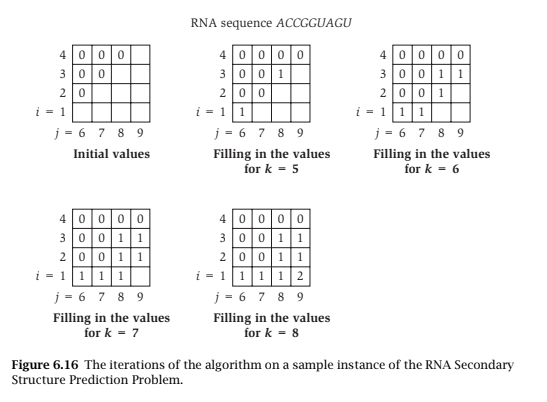
\includegraphics[]{figures/fig20.png}
\end{center}

\medskip
--------------------------------------------------------------------------------------------------------------------------
\medskip

\textbf{Algorithm}\\
Initialize opt(i,j) = 0 whenever i $\ge$ j-4\\
\texttt{For} k = 5, 6, ... , n-1\\
\texttt{For} i = 1, 2, ..., n-k\\
\texttt{Set} j = i + k\\
\texttt{Compute} opt(i,j) using the recurrence in (6.13)\\
\texttt{Endfor}\\
\texttt{Endfor}\\
\texttt{Return} opt(1,n)


\medskip
--------------------------------------------------------------------------------------------------------------------------
\medskip

It easy to bound the running time: there are O(n$^2$) sub-problems to solve, and evaluating the recurrence in (6.13) takes O(n) for each. Thus the running time is O(n$^3$). 

\section{Chapter 7: Network Flow}
One often uses graphs to model transportation networks—networks whose edges carry some sort of traffic and whose nodes act as “switches” passing traffic between different edges. Network models of this type have several ingredients: capacities on the edges, indicating how much they can carry; source nodes in the graph, which generate traffic; sink (or destination) nodes in the graph, which can “absorb” traffic as it arrives; and finally, the traffic itself, which is transmitted across the edges.\\

\subsection{The Max-Flow Problem and the Fold-Fulkerson Algorithm}

\textbf{Flow Networks} Let \emph{flow} be an abstract entity that is generated at source nodes, transmitted across edges, and absorbed at sink nodes. Formally, we’ll say that a flow network is a directed graph G = (V, E) with the following features:\\

\begin{enumerate}
    \item Associated with each edge e is a capacity, which is a non-negative number that we denote c$_e$.
    \item There is a single source node s $\in$ V
    \item There is a single sink node t $\in$ V
\end{enumerate}

Nodes other than s and t will be called internal nodes. We will make some assumptions about the flow networks we deal with:\\

\begin{enumerate}
    \item First, no edge enters the source s and no edge leaves the sink t
    \item Second, there is at least one edge incident to each node
    \item Third, all capacities are integers
\end{enumerate}

These assumptions make things cleaner to think about, and while they eliminate few pathologies, they preserve essentially all the issues we want to think about.\\

\textbf{Defining Flow} Next we define what it means for our network to carry traffic, or flow. We say that an s-t flow is a function f that maps each edge e to a non-negative real number. The value of f(e) intuitively represents the amount of flow carried by an edge. A flow f has to satisfy two following properties:\\

\begin{enumerate}
    \item (Capacity conditions) For each e $\in$ E, we have 0 $\le$ f(e) $\le$ c$_e$.
    \item (Conservation conditions) For each node v other than s and t, we have\\
    \begin{center}
         $\sum_{e into v}^{}$ f(e) = $\sum_{e out of v}^{}$ f(e)
    \end{center}
\end{enumerate}

 $\sum_{e into v}^{}$ f(e) sums the flow value f(e) over all edges entering v. $\sum_{e out of v}^{}$ f(e) is the sum of flow values over all edges leaving node v. Thus the flow on an edge cannot exceed the capacity of the edge. For every node other than the source and the sink, the amount of flow entering must equal the amount of flow leaving.\\

 The value of a flow f, denoted v(f), is defined to be the amount of flow generated at the source:\\
 \begin{center}
     v(f) = $\sum_{e out of s}^{}$ f(e)
 \end{center}

 To make our notation more compact, we define f$^{out}$ (v) = $\sum_{e out of v}^{}$ f(e) and f$^{in}$ = $\sum_{e into v}^{}$ f(e). We can extend this to sets of vertices; if S $\subseteq$ V, we define f$^{out}$ (s) = $\sum_{e out of s}^{}$ f(e) and f$^{in}$ (v) = f$^{out}$ (v): and we can write v(f) = $f^{out}$ (s).\\

 \textbf{The Max-Flow Problem} Given a flow network, a natural goal is to arrange the traffic so as to make as efficient use as possible of the available capacity. Thus the basic algorithmic problem we will consider is the following: Given a flow network, find a flow of maximum possible value.\\

 Here is a basic "challenge" to the existence of large flows: supposed we divide the nodes of the graph into two sets, A and B, such that s $\in$ A and t $\in$ B. Intuitively, any flow that goes from s to t must cross from A into B at some point, and this thereby uses up some of the edge capacity from A to B. This suggests the each such "cut" of the graph puts bound on the maximum possible flow value. The max-flow algorithm will be intertwined with a proof that the max-flow value equals the minimum capacity of any division called the \emph{minimum cut}. Our algorithm will also find the minimum cut. Finding the minimum cut will be useful in finding the max-flow.\\

\subsubsection{Designing the Algorithm}
No solution to the max-flow fits into the paradigm of dynamic programming so we can go back to greedy. Supposed we have zero flow: f(e) = 0 for all e. Clearly this works. Now try to increase the flow by "pushing" flow along a path from s to t, up to the limits imposed by the edge capacities. Looking at the figure elow, we might choose the path {(s,u), (u,v), (v,t)} and increase the flow on each of these edges to 20 and leave f(e) = 0 for the other two.\\

\begin{center}
    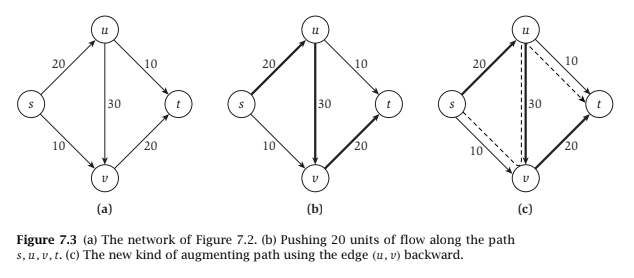
\includegraphics[]{figures/fig21.png}
\end{center}

Now, thinking about it, is 20 our maximum flow? No since its possible to construct a flow of 30. The problem is there is no s-t path on which you can directly push that flow without exceeding the some capacity. How would we achieve a flow of 30?\\

Essentially, we’d like to perform the following operation denoted by a dotted line in Figure 7.3(c). We push 10 units of flow along (s, v); this now results in too much flow coming into v. So we “undo” 10 units of flow on (u, v); this restores the conservation condition at v but results in too little flow leaving u. So, finally, we push 10 units of flow along (u, t), restoring the conservation condition at u. We now have a valid flow, and its value is 30. This is a general way of pushing flow:\\

\begin{enumerate}
    \item We can push forward on edges with leftover capacity
    \item We can push backwards on edges that are already carrying flow
    \item Pushing back on those edges, allows use to divert it in a different direction.
    \item We define this as a residual graph, which provides a systemic way to search for forward-backward flow.
\end{enumerate}

\textbf{The Residual Graph} Given a flow network G, and a flow f on G, we defined the residual graph G$_f$ of G with respect to f as:\\

\begin{center}
    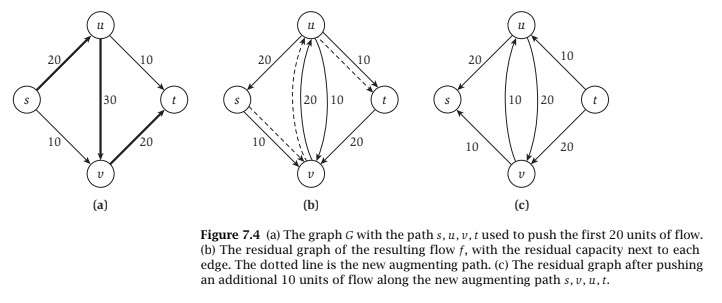
\includegraphics[]{figures/fig22.png}
\end{center}

\begin{enumerate}
    \item The node set of G$_f$ is the same as that of G
    \item For each edge e = (u,v) of G on which f(e) $\le$ c$_e$, there are c$_e$ - f(e) "leftover" units of capacity on which we could try pushing flow forward. So we include the edge e = (u,v) in G$_f$, with a capacity of c$_e$ - f(e). We will call edges included this way forward edges.
    \item For each edge e = (u,v) of G on which f(e) $>$ 0, there are f(e) units of flow that we can "undo" if we want to, by pushing flow backwards. So we include the edge e' = (u,v) in G$_f$, with a capacity of f(e). e' and e have the same ends, but reversed direction. We call these edges backward edges.
\end{enumerate}

\textbf{Augmenting Paths in a Residual Graph} Now we want to make precise the way in which we push flow from s to t in the residual graph. Let P be a simple s-t path in G$_f$, P only visits any node once. We define \texttt{bottleneck}(P,f) to be the minimum residual capacity of any edge on P, with respect to f. We now define the following operation \texttt{augment}(f,P), which yields a new flow f' in G. The result of augment(f,P) is a new flow f' in G, obtained by increasing and decreasing flow values on edges of P. \\

\medskip
--------------------------------------------------------------------------------------------------------------------------
\medskip

\textbf{augment(f,P)}\\
\texttt{Let} b = bottleneck(P,f)\\
\texttt{For} each edge (u,v) $\in$ P\\
\texttt{If} e = (u,v) is a forward edge then increase f(e) in G by b\\
\texttt{Else} ((u,v) is a backward edge, and let e = (u,v))\\
decrease f(e) in G by b\\
\texttt{Endif}\\
\texttt{Endfor}\\
\texttt{Return}(f)\\


\medskip
--------------------------------------------------------------------------------------------------------------------------
\medskip

This augmentation algorithm operation captures the type of forward and backward pushing flow that we discussed earlier. Now let's consider the following algorithm to compute s-t flow in G. This algorithm is caled \emph{Ford-Fulkerson Algorithm}. The algorithm is quite simple, however it is unlike whether the central \texttt{while} loop terminates, and whether the flow returned is a max-flow. The answer turns out to be fairly subtle.\\

\medskip
--------------------------------------------------------------------------------------------------------------------------
\medskip

\textbf{Max-Flow}\\
Initially f(e) = 0 for all e in G\\
\texttt{While} there is an s-t path in the residual graph G$_f$\\
\texttt{Let} P be a simple s-t path in G$_f$\\
f' = augment(f,P)\\
\texttt{Update} f to f'\\
\texttt{Update} the residual graph G$_f$ to be G$_f'$\\
\texttt{Endwhile}\\
\texttt{Return} f\\


\medskip
--------------------------------------------------------------------------------------------------------------------------
\medskip

\subsubsection{Analyzing the Algorithm}

\fbox{\begin{minipage}{12 cm}

\begin{center}
(7.2)\\
At every intermediate stage of the Ford-Fulkerson Algorithm, the flow values {f(e)} and the residual capacities of G$_f$ are integers.\\
\end{center}

\end{minipage}}\\

\medskip

\fbox{\begin{minipage}{12 cm}

\begin{center}
(7.3)\\
Let f be a flow in G, and let P be a simple s-t path in G$_f$. Then v(f') = v(f) + bottleneck(P,f); and since bottleneck(P,f) $>$ 0, we have v(f') $>$ v(f).\\
\end{center}

\end{minipage}}\\

\medskip

To prove termination, we need to be able to bound the max flow and that flow values strictly increase: 

\begin{enumerate}
    \item (7.3) Let f be a flow in G, and let P be a simple s-t path in G$_f$. Then v(f') = v(f) + \texttt{bottleneck}(P,f); and since \texttt{bottleneck}(P,f) $>$ 0, we have v(f') $>$ v(f). This means flow values strictly increase when we apply augmentation.
    \item One upper bound: if all the edges out of s could be completely saturated with flow, the flow value would be $\sum_{e out of s}$ c$_e$. Let C denote this sum, thus we have v(f) $\le$ C for all s-t flows. 
\end{enumerate}

\fbox{\begin{minipage}{12 cm}

\begin{center}
(7.4)\\
Suppose, all capacities in the flow network G are integers. Then the Ford-Fulkerson Algorithm terminates in at most C iterations of the \texttt{While} loop.\\
\end{center}

\end{minipage}}\\

\medskip

\fbox{\begin{minipage}{12 cm}

\begin{center}
(7.5)\\
Suppose, all capacities in the flow network G are integers. Then the Ford-Fulkerson Algorithm can be implemented to run in O(mC) time.\\
\end{center}

\end{minipage}}\\

\subsection{Max Flows and Minimum Cuts in a Network}
\subsubsection{Analyzing the Algorithm: Flows and Cuts}
Our next goal is to show that the flow that is returned by the Ford-Fulkerson Algorithm has the maximum possible value of any flow in G. Sometimes our previous upper bound is useful, but sometimes its very weak. We now use the notion of a "cut" to develop a much more general means of placing upper bounds on the max flow value.\\

Consider dividing the nodes of the graph into two sets, A and B such that s $\in$ A and t $\in$ B. The flow must cross from A to B somewhere, so formally we can say that a s-t cut is a partition (A,B) of the vertex set V such that s $\in$ A and t $\in$ B. The capacity of a cut (A,B), which be denoted as c(A,B) which is simply the sum of the capacities of all edges out of A:\\

\begin{center}
c(A,B) = $\sum_{e out of A}$ c$_e$
\end{center}

Cuts turn out to provide a natural upper bound on the flow values: We can make this precise via:\\

\fbox{\begin{minipage}{12 cm}

\begin{center}
(7.6)\\
Let f be any s-t flow, and (A,B) any s-t cut. Then v(f) = f$^{out}$(A) - f$^{in}$(A).
\end{center}

\end{minipage}}\\

\fbox{\begin{minipage}{12 cm}

\begin{center}
(7.7)\\
Let f be any s-t flow, and (A,B) any s-t cut. Then v(f) = f$^{in}$(B) - f$^{out}$(B)
\end{center}

\end{minipage}}\\

\fbox{\begin{minipage}{12 cm}

\begin{center}
(7.8)\\
Let f be any s-t flow, and (A,B) any s-t cut. Then v(f) $\le$ c(A,B)
\end{center}

\end{minipage}}\\

\subsubsection{Analyzing the Algorithm: Max Flow = Min Cut}
Let f$^-$ denote the flow returned by the Ford-Fulkerson Algorithm. We exhibit an s-t cut (A$^\ast$, B$^\ast$) for which v(f$^-$) = c(A$^*$, B$^*$). This establishes that f$^-$ has a max flow and (A$^*$, B$^*$) is a min capacity of any s-t cut. The algorithm terminates when flow f has no s-t path in G$_f$.\\

\fbox{\begin{minipage}{12 cm}

\begin{center}
(7.9)\\
If f is an s-t flow such that there is no s-t path in the residual grpah G$_f$, then there is an s-t cut (A$^*$, B$^*$) in G for which v(f) = c(A$^*$, B$^*$). Consequently, f has the maximum value of any flow in G, and (A$^*$, B$^*$) has the minimum capacity of any s-t cut in G.
\end{center}

\end{minipage}}\\

\begin{center}
    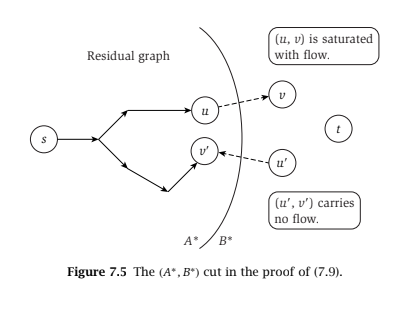
\includegraphics[]{figures/fig23.png}
\end{center}

\fbox{\begin{minipage}{12 cm}

\begin{center}
(7.10)\\
The flow f$^-$ returned by the Ford-Fulkerson Algorithm is a max flow.
\end{center}

\end{minipage}}\\

\fbox{\begin{minipage}{12 cm}

\begin{center}
(7.11)\\
Given a flow f of a max value, we can compute an s-t cut of minimum capacity in O(m) time.
\end{center}

\end{minipage}}\\

\fbox{\begin{minipage}{12 cm}

\begin{center}
(7.12)\\
In every flow network, there is a flow f and a cut (A,B) so that v(f) = c(A,B).
\end{center}

\end{minipage}}\\

\fbox{\begin{minipage}{12 cm}

\begin{center}
(7.13)\\
In every flow network, the maximum value of an s-t flow is equal to the minimum capacity of an s-t cut.
\end{center}

\end{minipage}}\\

\fbox{\begin{minipage}{12 cm}

\begin{center}
(7.14)\\
If all capacities in the flow network are integers, then there is a max flow f for which every flow value f(e) is an integer.
\end{center}

\end{minipage}}\\

\subsubsection{Preflow-Push Max Flow Algorithm}
Algorithms based on augmenting paths maintain a flow f, and use the augment procedure to increase the value of the flow. By way of contrast, the Preflow-Push Algorithm will, in essence, increase the flow on an edge-by-edge basis.\\

\textbf{Preflows} We say that an s-t preflow is a function f that maps each edge e to a non-negative real number. A preflow f must satisfy the capacity conditions:\\

\begin{enumerate}
    \item For each e $\in$ E, we have 0 $\le$ f(e) $\le$ c$_e$\\
    In place of conservation conditions, we only require inequalities. Each node other than s must have at least as much flow entering as leaving
    \item For each node v other than the source s, we have:\\
    $\sum_{e into v}$ f(e) $\ge$ $\sum_{e out of v}$f(e)\\
    We will call the difference the excess of preflow at node v: e$_f$(v) = $\sum_{e into v}$f(e) - $\sum_{e out of v}$f(e)
\end{enumerate}

\textbf{Preflows and Labeling} The Preflow-Push algorithm will maintain a preflow and work on converting preflow into flow. This algorithm is based on the physical intuition that flow naturally finds its way "downhill." The "heights" will be labeled h(v). We will say that a labeling h and an s-t preflow f are compatible if:\\

\begin{enumerate}
    \item (Source and sink conditions) h(t) = 0 and h(s) = n
    \item (Steepness conditions) For all edges (v,w) $\in$ E$_f$ in the residual graph, we have h(v) $\le$ h(w) + 1
\end{enumerate}

\begin{center}
    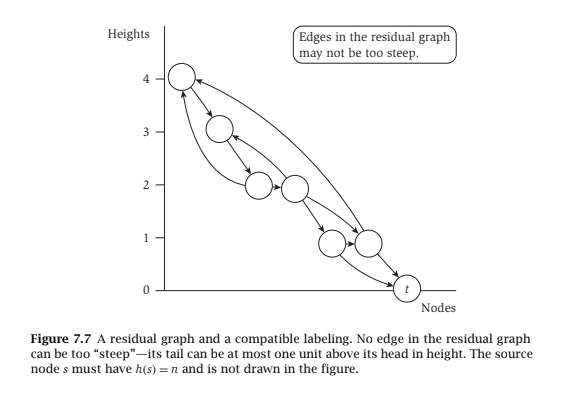
\includegraphics[]{figures/fig24.png}
\end{center}

Intuitively, the height difference n between the source and the sink is meant to ensure that the flow starts high enough to flow from s toward the sink t, while the steepness condition will help by making the descent of the flow gradual enough to make it to the sink. The key property of a compatible preflow is that there can be no s-t path in the residual graph\\

\fbox{\begin{minipage}{12 cm}

\begin{center}
(7.21)\\
If s-t preflow f is compatible with a labeling h, then there is no s-t path in the residual graph
\end{center}

\end{minipage}}\\

\fbox{\begin{minipage}{12 cm}

\begin{center}
(7.22)\\
If s-t flow f is compatible with a labeling h, then f is a flow of maximum value
\end{center}

\end{minipage}}\\

\fbox{\begin{minipage}{12 cm}

\begin{center}
(7.23)\\
The initial preflow f and labeling h are compatible
\end{center}

\end{minipage}}\\

\textbf{Pushing and Relabeling} Next we will discuss the steps the algorithm makes toward turning the preflow f into a feasible flow, while keeping it compatible with some labeling h. Consider any node v that has excess—that is, e$_f$(v) > 0. If there is any edge e in the residual graph G$_f$ that leaves v and goes to a node w at a lower height (note that h(w) is at most 1 less than h(v) due to the steepness condition), then we can modify f by pushing some of the excess flow from v to w. We will call this a push operation.

\medskip
--------------------------------------------------------------------------------------------------------------------------
\medskip

\textbf{push(f,h,v,w)}\\
\texttt{Applicable if} e$_f$(v) $>$ 0, h(w) $<$ h(v) and (v,w) $\in$ E$_f$\\
\texttt{If} e = (v,w) is a forward edge then\\
\texttt{let} $\delta$ = min(e$_f$(v), c$_e$ - f(e)) and\\
increase f(e) by $\delta$\\
\texttt{If} (v,W) is a backward edge then\\
\texttt{let} e = (w,v), $\delta$ = min(e$_f$(v), f(e)) and\\
decrease f(e) by $\delta$\\
\texttt{Return} (f,h)\\

\medskip
--------------------------------------------------------------------------------------------------------------------------
\medskip

If we cannot push the excess of v along any edge leaving v, then we will need to raise v's height. We will call this a \emph{relabel} operation!\\

\medskip
--------------------------------------------------------------------------------------------------------------------------
\medskip

\textbf{relabel(f,h,v)}\\
\texttt{Applicable if} e$_f$(v) $>$ 0 and\\
for all edges (v,w) $\in$ E$_f$ we have h(w) $\ge$ h(v)\\
Increase h(v) by 1\\
\texttt{Return} (f,h)\\

\medskip
--------------------------------------------------------------------------------------------------------------------------
\medskip

\medskip
--------------------------------------------------------------------------------------------------------------------------
\medskip

\textbf{Preflow-Push}\\
\texttt{Initially} h(v) = 0 for all v $\neq$ s and h(s) = n and\\
f(e) = c$_e$ for all e = (s,v) and f(e) = 0 for all other edges\\
\texttt{While} there is a node v $\neq$ t with excess e$_f$(v) $>$ 0\\
\texttt{Let} v be a node with excess\\
\texttt{If} there is w such that push(f,h,v,w) can be applied then\\
push(f,h,v,w)\\
\texttt{Else}\\
relabel(f,h,v)\\
\texttt{Endwhile}\\
\texttt{Return}(f)\\

\medskip
--------------------------------------------------------------------------------------------------------------------------
\medskip

\subsubsection{Analyzing the Algorithm}
For an implementation of the algorithm, we will have to specify which node with excess to choose, and how to efficiently select an edge on which to push. However, it is clear that each iteration of this algorithm can be implemented in polynomial time.\\

\fbox{\begin{minipage}{12 cm}

\begin{center}
(7.24)\\
Throughout the Preflow-Push Algorithm:
\begin{enumerate}
    \item the labels are non-negative integers;
    \item f is a preflow, and if the capacities are integral, then the preflow f is integral; and
    \item the preflow f and labeling h are compatible
\end{enumerate}
If the algorithm returns a preflow f, then f is a flow of maximum value.
\end{center}

\end{minipage}}\\

\fbox{\begin{minipage}{12 cm}

\begin{center}
(7.25)\\
Let f be a preflow, If the node v has excess, then there is a path in G$_f$ from v to the source s.
\end{center}

\end{minipage}}\\

\fbox{\begin{minipage}{12 cm}

\begin{center}
(7.26)\\
Throughout the algorithm, all nodes have h(v) $\le$ 2n-1.
\end{center}

\end{minipage}}\\

\fbox{\begin{minipage}{12 cm}

\begin{center}
(7.27)\\
Throughout the algorithm, each node is relabeled at most 2n-1 times, and the total number of relabeling operations is less than 2n$^2$.
\end{center}

\end{minipage}}\\

\fbox{\begin{minipage}{12 cm}

\begin{center}
(7.28)\\
Throughout the algorithm, the number of saturating push operations is at most 2nm.
\end{center}

\end{minipage}}\\

\fbox{\begin{minipage}{12 cm}

\begin{center}
(7.29)\\
Throughout the algorithm, the number of non-saturating push operations is at most 2n$^2$m.
\end{center}

\end{minipage}}\\

\begin{center}
    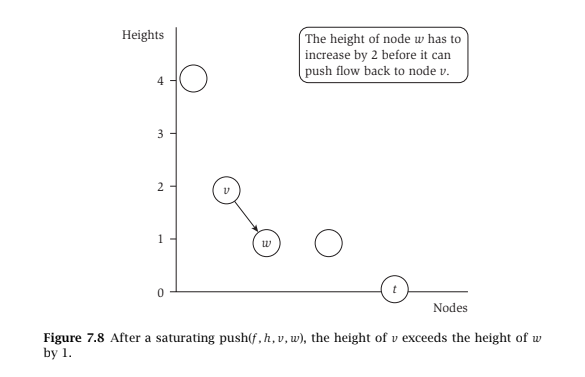
\includegraphics[]{figures/fig25.png}
\end{center}

\subsubsection{Extension: Improving Algorithm}

\fbox{\begin{minipage}{12 cm}

\begin{center}
(7.30)\\
If at each step we choose the node with excess at maximum height, then the number of non-saturating push operations throughout the algorithm is at most 4n$^3$.
\end{center}

\end{minipage}}\\

\subsubsection{Implementing Preflow-Push}
Maintaining a few simple data structures will allow us to effectively implement the operations of the algorithm in constant time each, and overall to implement the algorithm in time O(mn) plus the number of non-saturating push operations. Hence the generic algorithm will run in O(mn$^2$) time, while the version that always selects the node at maximum height will run in O(n$^3$) time.\\

\begin{enumerate}
    \item Maintain all nodes with excess on a simple list
    \item Maintain a linked list of all nodes with excess at every possible height (in order to select a node with max height H)
    \item Whenever a nodes gets relabeled, it remains a node with max height H
    \item If node v was at max height, then the new node at max height will also be at H.
    \item If no node at H has excess, then the max height will be H-1 -> push from H to H-1
    \item Now we select a node v and edge (v,w) and apply push (or relabel)
    \item To be able to select an edge quickly, we will use the adjacency list representation of the graph. More precisely, we will maintain, for each node v, all possible edges leaving v in the residual graph in a linked list and with each edge we keep its capacity and flow.
    \item We have two copies of each edge in our data structure, forward and backward
    \item These two copies will have pointers to each other and updates done in O(1) time.
    \item Select edges leaving v for pushing based on node v's list
    \item Maintain a pointer: current(v)
    \item If node v no longer has excess after a non-saturating push out of v, current(v) will stay at this edge
    \item After a saturating push out of v, we advance current(v) to the next edge
    \item The key observation is that, after advancing the pointer current(v) from an edge (v, w), we will not want to apply push to this edge again until we relabel v.
\end{enumerate}

\fbox{\begin{minipage}{12 cm}

\begin{center}
(7.31)\\
After current(v) is advanced from an edge (v,w), we cannot apply push to this edge until v gets relabeled.
\end{center}

\end{minipage}}\\

\fbox{\begin{minipage}{12 cm}

\begin{center}
(7.32)\\
When current(v) reaches the end of the list for v, the relabel operation can be applied to node v.
\end{center}

\end{minipage}}\\

\fbox{\begin{minipage}{12 cm}

\begin{center}
(7.33)\\
The running time of the Preflow-Push algorithm, implemented using the above data structures, is O(mn) + O(1) for each non-saturating push operation. In particular, the generic Preflow-Push runs in O(n$^2$m) time, while the version where we always select the node at max height runs in O(n$^3$) time.
\end{center}

\end{minipage}}\\

\textbf{Summary}
\begin{enumerate}
    \item Generic Preflow-Push: O(n$^2$m)
    \item Preflow-Push selecting max height: O(n$^3$)
    \item Preflow-Push using pointer and linked list:  O(mn) + O(1) 
\end{enumerate}

\section{Chapter 8: NP and Computational Intractability}
 Thus far we have came up with efficient algorithms for solving problems in polynomial time. There exists extremely hard problems in which we do not have algorithms in polytime to solve these problems, therefore no polytime algorithms exist for these kinds of problems. However there also exists a large set of problems that fall in a "gray area" in which it has been proven that if a polynomial-time algorithm existed for them, then a polynomial-time algorithm would exist for ALL of them. These are the NP-complete problems. There are literally thousands of NP-complete problems, arising in numerous areas, and the class seems to contain a large fraction of the fundamental problems whose complexity we can’t resolve. So the formulation of NP-completeness, and the proof that all these problems are equivalent, is a powerful thing: it says that all these open questions are really a single open question, a single type of complexity that we don’t yet fully understand.

 \subsection{Polynomial-Time Reductions}
 The way we go about these problems is proving polynomial time reducibility. Y $\le$$_p$ X means "Y is polynomial time reducible to X." An important consequence of this is:\\

 Suppose Y $\le$$_p$ X and there actually exists a polynomial-time algorithm to solve X. Then our specialized black box for X is actually not valuable. It now becomes an algorithm that involves polynomial numbers of steps, polynomial number of calls to a subroutine that runs in polynomial time, therefore proving:\\

 \fbox{\begin{minipage}{12 cm}

\begin{center}
(8.1)\\
Suppose Y $\le$$_p$ X. If X can be solved in polynomial time, then Y can be solved in polynomial time.
\end{center}

\end{minipage}}\\

An example of this was when looking at Ford-Fulkerson's Algorithm to solve Max Flow. Since Max Flow can be solved in polynomial time, we can also conclude that Bipartite Matching could also be solved in polynomial time. However, for this chapter we will use (8.1) to establish the computational intractability of various problems.\\

 \fbox{\begin{minipage}{12 cm}

\begin{center}
(8.2)\\
Suppose Y $\le$$_p$ X. If Y cannot be solved in polynomial time, then X cannot be solved in polynomial time.
\end{center}

\end{minipage}}\\

\subsubsection{A First Reduction: Independent Set and Vertex Cover}
\textbf{Independent Set} Let’s review the formulation of Independent Set, because we’re going to add one wrinkle to it. Recall that in a graph G = (V, E), we say a set of nodes S $\subseteq$ V is independent if no two nodes in S are joined by an edge. It is easy to find small independent sets in a graph (for example, a single node forms an independent set); the hard part is to find a large independent set, since you need to build up a large collection of nodes without ever including two neighbors.\\

We originally posed the problem of finding the largest independent set in a graph G. It will be more convenient to work with problems that have a yes/no answer:\\

\emph{Given a graph G and a numb k, does G contain an independent set of size at least k?}\\

For given a graph G on n nodes, we simply solve the decision version of Independent Set for each k; the largest k for which the answer is “yes” is the size of the largest independent set in G. (And using binary search, we need only solve the decision version for O(log n) different values of k.) This simple equivalence between decision and optimization will also hold in the problems we discuss below.\\

\textbf{Vertex Cover} Now lets illustrate the basic strategy for another fundamental graph problem known as \emph{Vertex Cover}. Given a graph G = (V, E), we say that a set of nodes S $\subseteq$ V is a vertex cover if every edge e $\in$ E has at least one end in S. In a vertex cover, the vertices do the “covering,” and the edges are the objects being “covered.” Now, it is easy to find large vertex covers in a graph (for example, the full vertex set is one); the hard part is to find small ones. We formulate the Vertex Cover Problem as follows: \\

\emph{Given a graph G and a number k, does G contain a vertex cover of size at most k?}\\

We don't know how to solve either Independent Set or Vertex Cover in polynomial time; but what can we say about their relative difficulty? We now
show that they are equivalently hard, by establishing that Independent Set $\le$$_p$ Vertex Cover and also that Vertex Cover $\le$$_p$ Independent Set.\\

 \fbox{\begin{minipage}{12 cm}

\begin{center}
(8.3)\\
Let G = (V,E) be a graph. Then S is an independent set if and only if its complement V - S is a vertex cover.
\end{center}

\end{minipage}}\\

\textbf{Proof}
First, supposed that S is an independent set. Consider an arbitrary edge e = (u,v). Since S is independent, it cannot be the case that both u and v are in S; so one of them must be in V - S. It follows that every edge has at least one end in V - S, and so V - S is a vertex cover.\\

Conversely, suppose that V - S is a vertex cover. Consider any two nodes u and v in S. If they were joined by edge e, then neither end of e would lie in V - S, contradicting our assumption that V - S is a vertex cover. It follows that no two nodes in S are joined by an edge, and so S in an independent set.\\

 \fbox{\begin{minipage}{12 cm}

\begin{center}
(8.4)\\
Independent Set $\le$$_p$ Vertex Cover
\end{center}

\end{minipage}}\\

 \fbox{\begin{minipage}{12 cm}

\begin{center}
(8.5)\\
Vertex Cover $\le$$_p$ Independent Set
\end{center}

\end{minipage}}



\subsubsection{Reducing to General Case: Vertex Cover to Set Cover} Independent Set and Vertex Cover represent two different genres of problems:

\begin{enumerate}
    \item Independent Set can be viewed as a packing problem: The goal is to “pack in” as many vertices as possible, subject to conflicts (the edges) that try to prevent one from doing this.
    \item Vertex Cover, on the other hand, can be viewed as a covering problem: The goal is to parsimoniously “cover” all the edges in the graph using as few vertices as possible.
\end{enumerate}

\textbf{Set Cover} There is a more general covering problem, Set Cover, in which you seek to cover an arbitrary set of objects using a collection of smaller sets. We can phrase Set Cover as follows:\\

\emph{Given a set U of n elements, a collection S$_1$,..., S$_m$ of subsets of U, and a number k, does there exist a collection of at most k of these sets whose union is equal to all of U?}\\

Intuitively, it feels like Vertex Cover is a special case of Set Cover: in the latter case, we are trying to cover an arbitrary set using arbitrary subsets, while in the former case, we are specifically trying to cover edges of a graph using sets of edges incident to vertices. In fact, we can show the following reduction.\\

\fbox{\begin{minipage}{12 cm}

\begin{center}
(8.6)\\
Vertex Cover $\le$$_p$ Set Cover
\end{center}

\end{minipage}}\\

\textbf{Set Packing} Just as Set Cover is a natural generalization of Vertex Cover, there is a natural generalization of Independent Set as a packing problem for arbitrary sets. Specifically, we define the Set Packing Problem as follows:\\

\emph{Given a set U of n elements, a collection S$_1$,..., S$_m$ of subsets of U, and a number k, does there exist a collection of at least k of these sets with the property that no two of them intersect?}\\

\fbox{\begin{minipage}{12 cm}

\begin{center}
(8.7)\\
Independent Set $\le$$_p$ Set Packing
\end{center}

\end{minipage}}\\

\subsection{Reductions via "Gadgets": The SAT Problem}
We now introduce a somewhat more abstract set of problems, which are formulated in Boolean notation. As such, they model a wide range of problems in which we need to set decision variables so as to satisfy a given set of constraints.\\

\subsubsection{The SAT and 3-SAT Problems}
Suppose we are given a set X of n Boolean variables x$_1$,..., x$_n$; each can take the value 0 or 1. By a term over X, we mean one of the variables x$-i$ or its negation x$_{i}^{-}$. Finally, a clause is simply a disjunction of distinct terms.\\

\begin{center}
    \emph{t$_1$ $\vee$ t$_2$ $\vee$ ... $\vee$ t$_l$}
\end{center}

We now formalize what it means for an assignment of values to satisfy a collection of clauses. A truth assignment for X is an assignment of the value 0 or 1 to each x$_{i}^{*}$; An assignment satisfies a clause C if it causes C to evaluate to 1 under the rules of Boolean logic; this is equivalent to requiring that at least one of the terms in C should receive the value 1. An assignment satisfies a collection of clauses C$_1$,..., C$_k$ if it causes all of the C$_i$ to evaluate to 1; in other words, if it causes the conjunction:\\

\begin{center}
    \emph{C$_1$ $\wedge$ C$_2$ $\wedge$ ... $\wedge$ C$_k$}
\end{center}

\textbf{SAT} We can now state the Satisfiability Problem, also referred to as SAT: \\

\begin{center}
    \emph{Given a set of clauses C$_1$,..., C$_k$ over a set of variables X = (x$_1$,..., x$_n$), does there exist a satisfying truth assignment?}
\end{center}

\textbf{3-SAT} There is a special case of SAT that will turn out to be equivalently difficult and is somewhat easier to think about; this is the case in which all clauses contain exactly three terms (corresponding to distinct variables). We call this problem 3-Satisfiability, or 3-SAT:\\

\begin{center}
    \emph{Given a set of clauses C$_1$,..., C$_k$ each of length 3, over a set of variables X = (x$_1$,..., x$_n$), does there exist a satisfying truth assignment?}
\end{center}

Satisfiability and 3-Satisfiability are really fundamental combinatorial search problems; they contain the basic ingredients of a hard computational problem in very “bare-bones” fashion. We have to make n independent decisions (the assignments for each xi) so as to satisfy a set of constraints. There are several ways to satisfy each constraint in isolation, but we have to arrange our decisions so that all constraints are satisfied simultaneously.\\

\subsubsection{Reducing 3-SAT to Independent Set}
3-SAT is about setting Boolean variables in the presence of constraints, while Independent Set is about selecting vertices in a graph. To solve an instance of 3-SAT using a black box for Independent Set, we need a way to encode all these Boolean constraints in the nodes and edges of a graph, so that satisfiability corresponds to the existence of a large independent set.\\

\textbf{Proof} We have a black box for Independent Set and want to solve an instance of 3-SAT consist of variables X = {x$_1$,...,x$_n$} and clauses C$_1$,...,C$_k$. The key to thinking about the reduction is to realize that there are two conceptually distinct ways of thinking about an instance of 3-SAT:\\

\begin{center}
    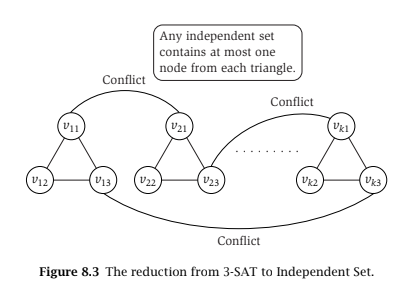
\includegraphics[]{figures/fig26.png}
\end{center}

\begin{enumerate}
    \item One way to picture the 3-SAT: You have to make an independent 0/1 decision for each of the n variables, and you succeed if you manage to achieve one of three ways of satisfying each clause.
    \item A different way: You have to choose one term from each clause, and then find a truth assignment that causes all these terms to evaluate to 1, thereby satisfying all clauses. So you succeed if you can select a term from each clause in such a way that no two selected terms "conflict." We say two terms conflict if one is equal to a variable x$_i$ and the other is equal to its negation x$_{i}^{-}$. If we avoid conflicting terms, we can find a truth assignment that makes the select terms from each clause evaluate to 1.
\end{enumerate}

Before proceeding, consider what the independent sets of size k look like in this graph: Since two vertices cannot be selected from the same triangle, they consist of all ways of choosing one vertex from each of the triangles.\\

\begin{enumerate}
    \item Let’s claim, precisely, that the original 3-SAT instance is satisfiable if and only if the graph G we have constructed has an independent set of size at least k. First, if the 3-SAT instance is satisfiable, then each triangle in our graph contains at least one node whose label evaluates to 1.
    \item Let S be a set consisting of one such node from each triangle. We claim S is independent; for if there were an edge between two nodes u, v $\in$ S, then the labels of u and v would have to conflict; but this is not possible, since they both evaluate to 1.
    \item Now, we claim that there is a truth assignment v for the variables in the 3-SAT instance with the property that the labels of all nodes in S evaluate to 1.
    \item For each variable x$_i$, if neither x$_i$ nor x$_{i}^{-}$ appears as a label of a node in S, then we arbitrarily set v(x$_i$) = 1.
    \item If one had a label on either x$_i$ or x$_{i}^{-}$, then S would not be an independent set since something would connect them.
    \item By constructing v in this way, all labels of nodes in S will evaluate to 1.
    \item Since G has an independent set of size at least k if and only if the original 3-SAT instance is satisfiable, the reduction is complete.
\end{enumerate}

We can conclude that:\\

\fbox{\begin{minipage}{12 cm}

\begin{center}
(8.8)\\
3-SAT $\le$$_p$ Independent Set
\end{center}

\end{minipage}}\\

\subsection{Transitivity}
The reduction we proved is also transitive across relations.\\

\fbox{\begin{minipage}{12 cm}

\begin{center}
(8.9)\\
If Z $\le$$_p$ Y, and Y $\le$$_p$ X, then Z $\le$$_p$ X
\end{center}

\end{minipage}}\\

\subsection{NP: A Class of Problems}
We define NP to be the set of all problems for which there exists an efficient certifier. We define a efficient certifier 'B' as:\\

\begin{enumerate}
    \item B is a polynomial-time algorithm that takes two input arguments s and t.
    \item There is a polynomial function p so that for every string s, we have x $\in$ X if and only if there exists a string t such that $\lvert t \rvert$ $\le$ p($\lvert s \rvert$) and B(s,t) = yes
\end{enumerate}

One thing we can immediately observe for NP:\\

\fbox{\begin{minipage}{12 cm}

\begin{center}
(8.10)\\
P $\subseteq$ NP
\end{center}

\end{minipage}}\\

\textbf{Proof} Consider a problem X $\in$ P; this means that there is a polynomial-time algorithm A that solves X. To show that X $\in$ NP, we must show that there is an efficient certifier B for X.\\

This is very easy; we design B as follows. When presented with the input pair (s, t), the certifier B simply returns the value A(s). (Think of B as a very “hands-on” manager that ignores the proposed proof t and simply solves the problem on its own.) Why is B an efficient certifier for X? Clearly it has polynomial running time, since A does. If a string s $\in$ X, then for every t of length at most p($\lvert s \rvert$), we have B(s,t) = no.\\

Now, we can easily check that the problems introduced in the first two sections belong to NP: it is a matter of determining how an efficient certifier for each of them will make use of a "certificate" string t:\\

\begin{enumerate}
    \item For the 3-Satisfiability Problem, the certificate t is an assignment of truth values to the variables; the certifier B evaluates the given set of clauses with respect to this assignment.
    \item For the Independent Set Problem, the certificate t is the identity of a set of at least k vertices; the certifier B checks that, for these vertices, no edge joins any pair of them.
    \item For the Set Cover Problem, the certificate t is a list of k sets from the given collection; the certifier checks that the union of these sets is equal to the underlying set U.
\end{enumerate}

Yet we cannot prove that any of these problems require more than polynomial time to solve. Indeed, we cannot prove that there is any problem in NP that does not belong to P. So in place of a concrete theorem, we can only ask a question:\\

\begin{center}
    \emph{Is there a problem in NP that does not belong to P? Does P = NP?}
\end{center}

\subsection{NP-Complete Problems}
In the absence of progress on the P = NP question, people have turned to a related but more approachable question: What are the hardest problems in NP? The most natural way to define "hardest" problem is via two properties:\\

\begin{enumerate}
    \item X $\in$ NP
    \item For all Y $\in$ NP, Y $\le$$_p$ X
\end{enumerate}

In other words, we require every problem in NP can reduced to X. We will call such an X an NP-complete problem.\\

\fbox{\begin{minipage}{12 cm}

\begin{center}
(8.7)\\
Suppose X is an NP-complete problem. Then x is solvable in polynomial time if and only if P = NP
\end{center}

\end{minipage}}\\

\textbf{Proof} Clearly, if P = NP, then X can be solved in polynomial time since it belongs to NP. Converse, suppose that X can be solved in polynomial time. If Y is any other problem in NP,then Y $\le$$_p$ X, it follows that Y can be solved in polynomial time. Hence NP $\subseteq$ P.\\

\subsection{Circuit Satisfiability: A First NP-Complete Problem}
To prove a problem is NP-complete, one must show how it could encode any problem in NP. This is a much trickier matter. In 1971, Cook and Levin independently showed how to do this for very natural problems in NP. Maybe the most natural problem choice for a first NP-complete problem is the following Circuit Satisfiability Problem.\\

To specify this problem, we need to make precise what we mean by a circuit. Consider the standard Boolean operators that we used to define the Satisfiability Problem: AND, OR, and NOT. Our definition of a circuit is designed to represent a physical circuit built out of gates that implement these operators. Thus we define a circuit K to be a labeled, directed acyclic graph.\\

\begin{enumerate}
    \item The sources in K (the nodes with no incoming edges) are labeled either with one of the constants 0 or 1, or with the name of a distinct variable. The nodes of the latter type will be referred to as the inputs to the circuit.
    \item Every other node is labeled with one of the Boolean operators AND, OR, or NOT; nodes labeled with AND or OR will have two incoming edges, and nodes labeled with NOT will have one incoming edge.
    \item There is a single node with no outgoing edges, and it will represent the output: the result that is computed by the circuit.
\end{enumerate}

\begin{center}
    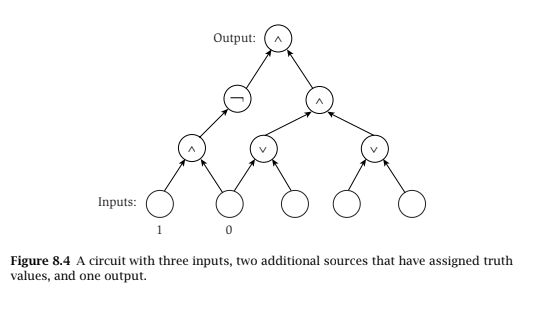
\includegraphics[]{figures/fig27.png}
\end{center}

Now, the Circuit Satisfiability Problem is the following. We are given a circuit as input, and we need to decide whether there is an assignment of values to the inputs that causes the output to take the value 1. (If so, we will say that the given circuit is satisfiable, and a satisfying assignment is one that results in an output of 1.).\\

\fbox{\begin{minipage}{12 cm}

\begin{center}
(8.13)\\
Circuit Satisfiability is NP-complete
\end{center}

\end{minipage}}\\

\fbox{\begin{minipage}{12 cm}

\begin{center}
(8.14)\\
If Y is an NP-complete problem, and X is a problem in NP with the property that Y $\le$$_p$ X, then X is NP-complete
\end{center}

\end{minipage}}\\

\fbox{\begin{minipage}{12 cm}

\begin{center}
(8.15)\\
3-SAT is NP-complete
\end{center}

\end{minipage}}\\

\fbox{\begin{minipage}{12 cm}

\begin{center}
(8.16)\\
All of the following problems are NP-complete: Independent Set, Set Packing, Vertex Cover, and Set Cover
\end{center}

\end{minipage}}\\

\subsection{General Strategy for Proving NP}
\begin{enumerate}
    \item Prove that X $\in$ NP.
    \item Choose a problem Y that is known to be NP-complete
    \item Prove that Y $\le$$_p$ X.
\end{enumerate}

We noticed earlier that most of our reductions Y $\le$$_p$ X consist of transforming a given instance of Y into a single instance of X with the same answer. This is a particular way of using a black box to solve X; in particular, it requires only a single invocation of the black box. When we use this style of reduction, we can refine the strategy above to the following outline of an NP-completeness proof.\\

\begin{enumerate}
    \item Prove that X $\in$ NP
    \item Choose a problem Y that is known to be NP-complete
    \item Consider an arbitrary instance of s$_y$ of problem Y, and show how to construct, in polynomial time, an instance s$_x$ of problem X that satisfies the following properties:
    \begin{enumerate}
        \item If s$_y$ is a "yes" instance of Y, then s$_x$ is a "yes" instance of X.
        \item If s$_x$ is a "yes" instance of X, then s$_y$ is a "yes" instance of Y\\
        In other words, this establishes that s$_y$ and s$_x$ have the same answer
    \end{enumerate}
\end{enumerate}

There has been research aimed at understanding the distinction between polynomial-time reductions with this special structure—asking the black box a single question and using its answer verbatim—and the more general notion of polynomial-time reduction that can query the black box multiple times. (The more restricted type of reduction is known as a Karp reduction, while the more general type is known as a Cook reduction and also as a polynomial-time Turing reduction.) We will not be pursuing this distinction further here.

\subsection{Sequencing Problems}
Thus far we have seen problems that (like Independent Set and Vertex Cover) have involved searching over subsets of a collection of objects; we have also seen problems that (like 3-SAT) have involved searching over 0/1 settings to a collection of variables. Another type of computationally hard problem involves searching over the set of all permutations of a collection of objects.\\

\subsubsection{The Traveling Salesman Problem}
Probably the most famous such sequencing problem is the Traveling Salesman Problem. Consider a salesman who must visit n cities labeled v$_1$, v$_2$,..., v$_n$. The salesman starts in city v$_1$, his home, and wants to find a tour—an order in which to visit all the other cities and return home. His goal is to find a tour that causes him to travel as little total distance as possible.

\begin{center}
    \emph{Given a set of distances on n cities, and a bound D, is there a tour of length at most D?}
\end{center}

\subsubsection{The Hamiltonian Cycle Problem}
The Traveling Salesman Problem has a natural graph-based analogue, which forms one of the fundamental problems in graph theory. Given a directed graph G = (V, E), we say that a cycle C in G is a Hamiltonian cycle if it visits each vertex exactly once. In other words, it constitutes a “tour” of all the vertices, with no repetitions.

\begin{center}
    \emph{Given a directed graph G, does it contain a Hamiltonian cycle?}
\end{center}

\subsubsection{Proving Hamiltonian Cycle is NP-complete}
We now show that both these problems are NP-complete. We do this by first establishing the NP-completeness of Hamiltonian Cycle, and then proceeding to reduce from Hamiltonian Cycle to Traveling Salesman.\\

\textbf{Proof} We first show that Hamiltonian Cycle is in NP. Given a directed graph G = (V, E), a certificate that there is a solution would be the ordered list of the vertices on a Hamiltonian cycle. We could then check, in polynomial time, that this list of vertices does contain each vertex exactly once, and that each consecutive pair in the ordering is joined by an edge; this would establish that the ordering defines a Hamiltonian cycle. We now show that 3-SAT $\le$$_p$ Hamiltonian Cycle.\\

So consider an arbitrary instance of 3-SAT, with variables x$_1$,..., x$_n$ and clauses C$_1$,..., C$_k$. We must show how to solve it, given the ability to detect
Hamiltonian cycles in directed graphs. As always, it helps to focus on the essential ingredients of 3-SAT: We can set the values of the variables however we want, and we are given three chances to satisfy each clause.

\begin{center}
    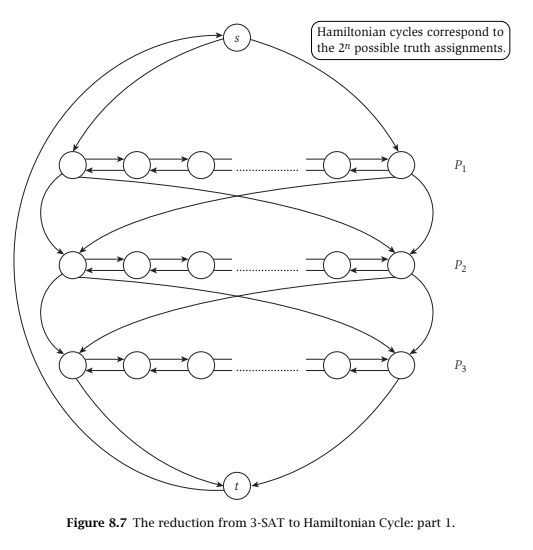
\includegraphics[]{figures/fig28.png}
\end{center}

\begin{center}
    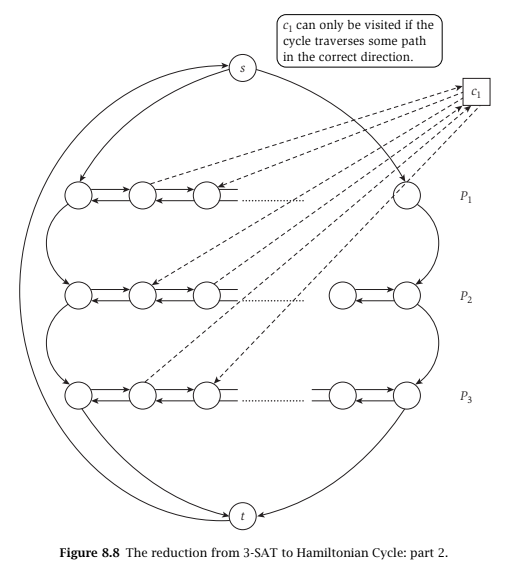
\includegraphics[]{figures/fig29.png}
\end{center}

This completes the construction of the graph G. Now, following our generic outline for NP-completeness proofs, we claim that the 3-SAT instance is satisfiable if and only if G has a Hamiltonian cycle. Having established that the 3-SAT instance is satisfiable if and only if G has a Hamiltonian cycle, our proof is complete. Therefore, we can conclude:\\

\fbox{\begin{minipage}{12 cm}

\begin{center}
(8.17)\\
Hamiltonian Cycle is NP-complete
\end{center}

\end{minipage}}\\

\fbox{\begin{minipage}{12 cm}

\begin{center}
(8.18)\\
Traveling Salesman is NP-complete
\end{center}

\end{minipage}}\\

\fbox{\begin{minipage}{12 cm}

\begin{center}
(8.19)\\
Hamiltonian Path is NP-complete
\end{center}

\end{minipage}}\\

\subsection{Partitioning Problems}
In the next two sections, we consider two fundamental partitioning problems, in which we are searching over ways of dividing a collection of objects into
subsets. Here we show the NP-completeness of a problem that we call 3- Dimensional Matching. In the next section we consider Graph Coloring, a problem that involves partitioning the nodes of a graph.\\

Consider the following 3-Dimensional Matching Problem:\\

\begin{center}
    \emph{Given disjoint sets X, Y, and Z, each of size n, and given a set T $\subseteq$ X × Y × Z of ordered triples, does there exist a set of n triples in T so that each element of X $\cup$ Y $\cup$ Z is contained in exactly one of these triples?}
\end{center}

\textbf{Proof} The arguments above can be turned quite easily into proofs that 3-Dimensional Matching $\le$$_p$ Set Cover and that 3-Dimensional Matching $\le$$_p$ Set Packing. But this doesn’t help us establish the NP-completeness of 3-Dimensional Matching, since these reductions simply show that 3-Dimensional Matching can be reduced to some very hard problems. What we need to show is the other direction: that a known NP-complete problem can be reduced to 3-Dimensional Matching.\\

\begin{center}
  \makebox[\textwidth]{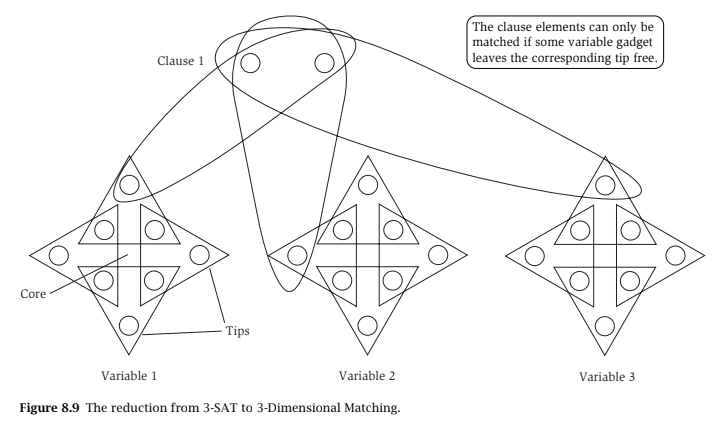
\includegraphics[width=\paperwidth]{figures/fig30.png}}
\end{center}


\fbox{\begin{minipage}{12 cm}

\begin{center}
(8.20)\\
3-Dimensional Matching is NP-complete
\end{center}

\end{minipage}}\\

\subsection{Other NP-Completes}

\textbf{Graph Coloring:}\\

\fbox{\begin{minipage}{12 cm}

\begin{center}
(8.22)\\
3-Coloring is NP-complete
\end{center}

\end{minipage}}\\

\textbf{Numerical Problems}\\

\fbox{\begin{minipage}{12 cm}

\begin{center}
(8.23)\\
Subset Sum is NP-complete
\end{center}

\end{minipage}}\\

\fbox{\begin{minipage}{12 cm}

\begin{center}
(8.23)\\
Scheduling with Release Times and Deadlines is NP-complete
\end{center}

\end{minipage}}\\

\section{Master Theorem}
To solve a recurrence relation running time you can use many different techniques. One popular technique is to use the Master Theorem also known as the Master Method. “ In the analysis of algorithms, the master theorem provides a solution in asymptotic terms (using Big O notation) for recurrence relations of types that occur in the analysis of many divide and conquer algorithms.”

\subsection{Theorem}
Let T(n) be a monotonically increasing function that satisfies:\\

\begin{center}
    T(n) = aT(n/b) + cn$^k$\\
    T(1) = c
\end{center}

where a $\ge$ 1, b $\ge$ 1, c $>$ 0. If f(n) $\in$ $\theta$(n$^d$), then:\\

\begin{enumerate}
    \item if a $<$ b$^d$: T(n) = $\theta$(n$^d$)
    \item if a = b$^d$: T(n) = $\theta$(n$^d$logn)
    \item if a $>$ b$^d$: T(n) = $\theta$(n$^{log_ba}$
\end{enumerate}

\subsubsection{Example 1}
Let T(n) = T(2n/3) + 1\\

How to solve:
\begin{enumerate}
    \item a = 1, since the coefficient in front of the inner T(n) is 1.
    \item b = 3/2 since its the inverse of the constant multiplier inside the function.
    \item d = 0, since n$^0$ results in 1.
    \item b$^d$ = (3/2)$^0$ which is equivalent to 1. And a = b$^d$. So our answer will be in the form of $\theta$(n$^d$logn)
    \item Plug in the known values: $\theta$(n$^0$logn) = $\theta$(logn)
    \item $\theta$(logn) is our answer.
\end{enumerate}

\subsubsection{Example 2}
Let T(n) = 2T(n/2) + nlogn\\

How to solve:
\begin{enumerate}
    \item a = 2, since the coefficient in front of the inner T(n) is 2.
    \item b = 2 since its the inverse of the constant multiplier inside the function.
    \item Solving for d is going to a different procedure for this problem since our f(n) isn't something as simple as a constant. So we can establish here that f(n) = nlogn
    \item f(n) nlogn = n$^1$ log$_1$n 
    \item d = 1, and k = 1 (k being the power of the log)
    \item We can find $\theta$ is = $\theta$(n$^{log_b^a}$log$^{k+1}$n)
    \item $\theta$(n$^1$log$^{2}$n) is our answer
\end{enumerate}

\end{document}
